\documentclass[lettersize,journal]{IEEEtran}
\usepackage{amsmath,amsfonts}
\usepackage{amsthm}
\usepackage{algorithmic}
\usepackage{algorithm}
\usepackage{array}
\usepackage[caption=false,font=normalsize,labelfont=sf,textfont=sf]{subfig}
\usepackage{textcomp}
\usepackage{stfloats,siunitx}
\usepackage{url}
\usepackage{verbatim}
\usepackage{graphicx}
\usepackage{cite}
\usepackage{multirow}
\usepackage{graphicx}   % Include graphics package
\usepackage{subcaption} % Include sub-caption package
\usepackage{float,booktabs} 
\usepackage{tikz,graphics,color,fullpage,float,epsf,caption,subcaption}
\usepackage{epsfig,epstopdf,lipsum,arydshln,amssymb,subfigure,multirow,microtype,lipsum,amsthm,amsfonts}
\hyphenation{op-tical net-works semi-conduc-tor IEEE-Xplore}
% updated with editorial comments 8/9/2021

\begin{document}

\title{Estimating Population Range by Recurring Online Chunk Bootstrap with Non-cumulative
Data in Streaming Data Environment}

\author{
\thanks{}}

%\author{Chidchanok Lursinsap${}^{1}$, Prem Jansawang${}^{2}$, Suphakant Phimoltares${}^{1}$ ~\IEEEmembership{}
        % <-this % stops a space
%\thanks{${}^{1}$Department of Mathematics and Computer Science, Faculty of Science, Chulalongkorn University, 
%Bangkok 10330, Thailand}% <-this % stops a space
%\thanks{${}^{2}$Department of Statistics, Faculty of Science, Khon Kaen University, Khon Kaen
%40002, Thailand}}

% The paper headers
%\markboth{Journal of \LaTeX\ Class Files,~Vol.~14, No.~8, August~2021}%
%{Shell \MakeLowercase{\textit{et al.}}: A Sample Article Using IEEEtran.cls for IEEE Journals}

\IEEEpubid{0000--0000/00\$00.00~\copyright~2021 IEEE}
% Remember, if you use this you must call \IEEEpubidadjcol in the second
% column for its text to clear the IEEEpubid mark.

\maketitle

\begin{abstract}

\end{abstract}

\begin{IEEEkeywords}
Article submission, IEEE, IEEEtran, journal, \LaTeX, paper, template, typesetting.
\end{IEEEkeywords}

\section{Introduction}
\IEEEPARstart{}{} 

The bootstrap method is a powerful and widely used statistical tool for estimating the uncertainty from finite samples of any parameter of interest, such as standard error, confidence intervals, and accuracy, etc.  Efron \cite{efron} introduced bootstrap methods as a generalization of the jackknife method, where the jackknife was mathematically expressed as a linear approximation of the bootstrap. Empirical results demonstrated that these methods are capable of estimating the standard error of complex estimators effectively. Efron and Tibshirani \cite{efron2} further explored the basic concepts and applications of bootstrap methods for estimating standard errors, confidence intervals, and other measures of statistical accuracy. For standard error estimation, data from a population is resampled with replacement to create multiple bootstrap samples, allowing for the calculation of statistics and their standard deviations for each sample. The results showed that bootstrap estimations provided reasonably accurate and efficient alignments with theoretical density curves. In terms of confidence intervals, several methods were empirically tested, showing that bootstrap confidence intervals can be more accurate than standard methods, particularly when the distribution of the statistic is non-normal. Achieving accurate results requires a sufficient number of bootstrap replications. Carpenter and Bithell \cite{carpenter} presented a practical guide for applying bootstrap confidence intervals in healthcare data, addressing when, which, and how to implement these methods. They assessed various bootstrap methods for confidence intervals across three families: pivotal, non-pivotal, and test-inversion. The experiments concluded that bootstrap confidence intervals are a suitable alternative when the assumptions of the underlying distribution do not hold, such as asymptotic normality, especially with small sample sizes or complex data structures. 

Range approximation in one-dimensional data plays an important role in statistics, data analysis, and computational sciences, aiming to estimate the interval between a dataset's minimum and maximum values.

\IEEEpubidadjcol



%\begin{figure*}[t]
%\centering
%\includegraphics[scale=0.6]{overview.eps}
%\vspace{-0.6in}
%\caption{Overview of proposed concept to identify actual number of clusters based on
%the observation of uniqueness of data distribution pattern and the finding of how the brain uses
%the past knowledge and experience to solve new problem.}  
%\label{overview}
%\end{figure*}

\section{Studied Problem and Objectives}

% Let a chunk of numeric data $({\bf C})$, a set of bins $({\bf B})$, and a set of numeric data $({\bf D})$ be defined as follows:

Let a chunk of numeric data $({\bf C})$, a bin $({\bf B})$, and a set of numeric data $({\bf D})$ be defined as follows:

\begin{enumerate}
%\item ${\bf D} = \{a \leq d_{j} \leq b \:\: | \:\: 1 \leq j \leq p\}$,
%for integer constants $p$, $a$, and $b$.
\item ${\bf D} = \{ d_j \in R| \: a \leq d_{j} \leq b \:\:{\rm for}\,\, j=1,2,\ldots,m$ 
$\,\, {\rm and}\,\, a, b, \in R\}$ 
\item The chunk ${\bf C}$ is divided into $n$ smaller chunks ${\bf c}_j \subset D$ for $j = 1,2,\ldots,n$ and $\cup_{i=1}^{n}{\bf c}_i \subset D.$  
%\item An integer data chunk ${\bf C}$ divided into $n$ smaller chunks, 
%${\bf C} = \{{\bf c}_{1}, \ldots, {\bf c}_{i}, \ldots, {\bf c}_{n} %\:\: | \:\: 1 \leq n < \infty\}$. 
%Each chunk has integers randomly taken from ${\bf D}$.
\item A set of bins ${\bf B}$ for containing all numeric values of a single chunk ${\bf c}_i$. There are two attributes, namely $v_i^{min}$ and $v_i^{max}$ such that for all $d_j \in {\bf c}_i$, $d_j \in [v_i^{min},v_i^{max}].$   
%\item A bin ${\bf B}$ for containing incoming all integers in each chunk. There are two attributes, 
%$v^{(min)}_{i}$ and $v^{(max)}_{i}$, defining the interval of integer values such that any integer 
%$v^{(min)}_{i} \leq d_{j} \leq v^{(max)}_{i}$ can be assigned to this %bin. 
\end{enumerate}
Each chunk ${\bf c}_{i}$ flows sequentially into the bin. If some values are less than $v^{(min)}$ or greater than $v^{(max)}$, then the width of ${\bf B}$ must be expanded. In the beginning, the size of the bin ${\bf B}$ is made large enough to contain all values in the first incoming chunk ${\bf c}_{1}$. Then, the size of ${\bf B}$ is occasionally expanded so that all values in the following incoming chunks can be assigned to the intervals of ${\bf B}$. The bin ${\bf B}$ is expanded if the values of some integers in some incoming chunks are either less than $v^{(min)}$ or greater 
than $v^{(max)}$. Therefore, the problem studied is defined as follows:  
Let $min({\bf D})$ and $max({\bf D})$ be the minimum and maximum values of ${\bf D}$. After capturing 
of integers in the first chunk, how to achieve the minimum number of expansions of ${\bf B}$ so that 


\begin{enumerate}
\item All incoming integers in the next other chunks can be assigned to ${\bf B}$.
\item $(min({\bf D}) - v^{(min)}_{1}) \geq 0$ is minimum.
\item $(v^{(max)}_{i} - max({\bf D})) \geq 0$ is minimum.
\end{enumerate}

\begin{figure}[!t]
\centering
%\resizebox{2.8in}{3.7in}{\includegraphics{example.eps}} 
\includegraphics[scale = 0.5]{example.eps} 
\caption{An example of studied problem.} 
\label{example}
\end{figure}

\IEEEpubidadjcol
Figure \ref{example} illustrates an example scenario of capturing chunks. There are 3 sequentially incoming
chunks containing these integers: ${\bf c}_{1} = \{7, 9, 23, 10\}$, ${\bf c}_{2} = \{2, 11, 1, 8\}$,
${\bf c}_{3} = \{25, 14, 6, 13\}$. After capturing ${\bf c}_{1}$, the values of left and right ends of
bin ${\bf B}$ are set to $v^{(min)} = 7$ and $v^{(max)} = 23$ and all data are discarded. Then, both ends 
are expanded in advance to $v^{(min)}= 4$ and $v^{(max)} = 25$, preparing for ${\bf c}_{2}$. 
When ${\bf c}_{2}$ enters, all integers except 2 can be captured because the left end value 
$v^{(min)}= 4$ is larger than 2. Thus, the left end $v^{(min)}$ is expanded to $v^{(min)} = 2$. 
No need to expand the right end. All data in ${\bf c}_{2}$ are discarded. Then, get ${\bf c}_{3}$.
The interval of ${\bf B}$ is large enough to capture all integers of ${\bf c}_{3}$. After capturing 
${\bf c}_{3}$, all integers are discarded. In this example, the number of expansions is 2, after chunks 1 
and 2. Generally, how to achieve the minimum number of expansions of ${\bf B}$ in advance so that both
expanded values are also minimum.

\subsection{Constraints}
The amount of integers in each ${\bf c}_{i}$ is denoted by $|{\bf c}_{i}|$. Bin $B$ can be considered 
as an interval having left end denoted by $L$ and right end denoted by $R$. The following constraints are imposed.
\begin{enumerate}
\item The probability of distribution of each integer $d_{j}$ in ${\bf c}_{i}$ is unknown.
\item $|{\bf c}_{i}| \neq |{\bf c}_{i+1}|$ or $|{\bf c}_{i}| = |{\bf c}_{i+1}|$.
\item After assigning all integers of ${\bf c}_{i}$ inside the bin, chunk ${\bf c}_{i}$ is completely 
discarded and never reentered the bin assignment.
\end{enumerate}

\section{Concept of Recurring Online Bootstrap in Streaming Environment with Unrecorded Data}

\begin{figure*}[!th]
\centering
\includegraphics[scale = 0.7]{concept-framework.eps} 
\caption{Framework.} 
\label{frame-work}
\end{figure*}

\subsection{Algorithm}
explain standard histogram first 

The algorithm has two phases. The first phase

\vspace{0.2in}
\noindent
{\bf Algorithm 1:} Capturing data chunks and expanding ${\bf B}$ when it is necessary. \\

\noindent
{\bf Input:} Stream of data chunks, ${\bf c}_{i}$ for $1 \leq i < \infty$. \\
{\bf Output:}

\vspace{0.2in}
\noindent
{\bf Phase 1:} Capturing ${\bf c}_{1}$ and get initial expansion of ${\bf B}$.

\begin{tabbing}
1.~~ \= Get ${\bf c}_{1}$ and set $total\_data = |{\bf c}_{1}|$. \\
2.~~ \> Let $v^{(min)} = \min({\bf c}_{1})$ and $v^{(max)} = \max({\bf c}_{1})$. \\
3.~~ \> Divide ${\bf B}$ into 8 equal sub-intervals ${\bf b}_{i}$ for $1 \leq i \leq 8$, \\
     \> each of size $(v^{(max)} - v^{(min)})/8$. \\
4.~~ \> Put the integers in ${\bf c}_{1}$ whose values are within \\
     \> sub-intervals ${\bf b}_{1}$ and ${\bf b}_{8}$ into these two sub-intervals. \\
5.~~ \> Count the number of integers in ${\bf b}_{1}$ and ${\bf b}_{8}$  \\
     \> and let $|{\bf b}_{1}|$ and $|{\bf b}_{8}|$ denote these numbers. \\
6.~~ \> Let $avg = (v^{(max)} + v^{(min)})/2$ be the middle value of \\
     \> ${\bf B}$. \\
7.~~ \> Find the types of probability distribution in list $P$ \\
     \> best fitting the data in ${\bf b}_{1}$, and ${\bf b}_{8}$ by using Algorithm \\
     \> 2.1 with $total\_data$, ${\bf b}_{1}$, and ${\bf b}_{8}$. \\
8.~~ \> Compute the standard number of integers in ${\bf b}_{1}$ \\
     \> denoted by $lstd$, and in ${\bf b}_{8}$ denoted by $rstd$. \\
     \> from the best fitted probability distribution by \\
     \> using Algorithm 2.2. \\
9.~~ \> ${\bf While}$ \= $|{\bf b}_{1}| > lstd$ or $|{\bf b}_{8}| > rstd$ ${\bf do}$ \\
10.~~ \>               \> ${\bf If}$ \= $|{\bf b}_{1}| > lstd$ ${\bf then}$ \\
11.~~\>               \>            \> Expand $v^{(min)}$ by using Algorithm 3 with \\
     \>               \>            \> all integers in ${\bf b}_{1}$. \\
12.~~\>               \> ${\bf EndIf}$ \\
13.~~\>               \> ${\bf If}$ \= $|{\bf b}_{8}| > rstd$ ${\bf then}$ \\
14.~~\>               \>            \> Expand $v^{(max)}$ by using Algorithm 4 with \\
     \>               \>            \> all integers in ${\bf b}_{8}$. \\
15.~~\>               \> ${\bf EndIf}$ \\
16.~~\>               \> Adjust the width of ${\bf b}_{1}$ and ${\bf b}_{8}$ by dividing ${\bf B}$ \\
     \>               \> into 8 equal sub-intervals ${\bf b}_{i}$ for $1 \leq i \leq 8$, \\
     \>               \> each of size $(v^{(max)} - v^{(min)})/8$. \\
17.~~\> ${\bf EndWhile}$ \\
18.~~\> Discard ${\bf c}_{1}$ and all integers in ${\bf b}_{1}$ and ${\bf b}_{8}$.
\end{tabbing}

\vspace{0.2in}
\noindent
{\bf Phase 2:} Capturing other ${\bf c}_{i}$ and determining the necessity of expanding ${\bf B}$.
\begin{tabbing}
1.~~ \= ${\bf while}$ \= there exists a new incoming chunk ${\bf c}_{i}$ ${\bf do}$ \\
2.~~ \>               \> $total\_data = total\_data + |{\bf c}_{i}|$. \\
x.~~ \>              \> ${\bf If}$ \,\=\,  $|{\bf b}_{1}| \geq min_B $  {\bf then}\\ 
x.~~ \>              \>           \> ${\bf B}_1 = \{\min({\bf c}_{i})\} \cup {\bf B}_1.$ \\
x.~~ \>              \>           \>  Apply ${\bf Alg.}$ 3 with ${\bf B}_1$ to get $v^{(min)}_B.$\\ 
x.~~ \>              \>           \> ${\bf If}$ \,\=\,  $v^{(min)} > v^{(min)}_B$\,\,${\bf then}$ \\
x.~~ \>              \>           \>   \> $v^{(min)} =v^{(min)}_B. $ \\
%x.~~ \>              \>           \> ${\bf Else}$\\
%x.~~ \>              \>           \>   \> $v^{(min)} =\frac{v^{(min)}+v^{(min)}_B}{2}. $ \\
x.~~ \>              \>           \> ${\bf EndIf}$\\
x.~~ \>              \> ${\bf Else}$ \\
x.~~ \>              \>  \> $v^{(min)} = \{\min({\bf c}_{i})\}.$\\
x.~~ \>              \> ${\bf EndIf}$\\
xx.~~ \>              \> ${\bf If}$ \,\=\,  $|{\bf b}_{8}| \geq min_B $  {\bf then}\\ 
x.~~ \>              \>           \> ${\bf B}_8 = \{\max({\bf c}_{i})\} \cup {\bf B}_8.$ \\
x.~~ \>              \>           \>  Apply ${\bf Alg.}$ 4 with ${\bf B}_8$ to get $v^{(max)}_B.$\\ 
x.~~ \>              \>           \> ${\bf If}$ \,\=\,  $v^{(max)} < v^{(max)}_B$\,\,${\bf then}$ \\
x.~~ \>              \>           \>   \> $v^{(max)} =v^{(max)}_B. $ \\
%x.~~ \>              \>           \> ${\bf Else}$\\
%x.~~ \>              \>           \>   \> $v^{(max)} =\frac{v^{(max)}+v^{(max)}_B}{2}. $ \\
x.~~ \>              \>           \> ${\bf EndIf}$\\
x.~~ \>              \> ${\bf Else}$ \\
x.~~ \>              \>  \> $v^{(max)} = \{\max({\bf c}_{i})\}.$\\
x.~~ \>              \> ${\bf EndIf}$\\
%3.~~ \>               \> ${\bf If}$ \> $\min({\bf c}_{i}) < v^{(min)}$ ${\bf then}$ \\
%4.~~ \>               \>          \> $v^{(min)} = \min({\bf c}_{i})$. \\
%5.~~ \>               \> ${\bf EndIf}$. \\
%6.~~ \>               \> ${\bf If}$ \= $v^{(max)} < \max({\bf c}_{i})$ ${\bf then}$ \\
%7.~~ \>               \>          \> $v^{(max)} = \max({\bf c}_{i})$. \\
%8.~~ \>               \> ${\bf EndIf}$. \\
9.~~ \>               \> Divide ${\bf B}$ into 8 equal sub-intervals ${\bf b}_{i}$ for \\
     \>               \> $1 \leq i \leq 8$, each of size $(v^{(max)} - v^{(min)})/8$. \\
10.~~\>               \> Put the integers in ${\bf c}_{i}$, whose values are within \\
     \>               \> sub-intervals ${\bf b}_{1}$ and ${\bf b}_{8}$, into these two \\
     \>               \> sub-intervals. \\
11.~~\>               \> Count the number of elements in ${\bf b}_{1}$ and ${\bf b}_{8}$  \\
     \>               \> and let $|{\bf b}_{1}|$ and $|{\bf b}_{8}|$ denote these numbers. \\
12.~~\>               \> Find the types of probability distribution in list $P$ \\
     \>               \> best fitting the data in ${\bf b}_{1}$, and ${\bf b}_{8}$ by using \\
     \>               \> Algorithm 2.1 with $total\_data$, ${\bf b}_{1}$, and ${\bf b}_{8}$. \\
13.~~\>               \> Compute the standard number of elements in ${\bf b}_{1}$ \\
     \>               \> denoted by $lstd$, and in ${\bf b}_{8}$ denoted by $rstd$ \\
     \>               \> from the best fitted probability distribution by \\
     \>               \> using Algorithm 2.2. \\
14.~~\>               \> ${\bf While}$ \= $|{\bf b}_{1}| > lstd$ or $|{\bf b}_{8}| > rstd$ ${\bf do}$ \\
x.~~\>               \>               \> $v^{(min)}_{old} = v^{(min)}$ \,\,and\,\, $v^{(max)}_{old} = v^{(max)}$ \\
15.~~\>               \>               \> ${\bf If}$ \= $|{\bf b}_{1}| > lstd$ ${\bf then}$ \\
16.~~\>               \>               \>            \> Expand $v^{(min)}$ by using Algorithm 3 \\
     \>               \>               \>            \> with all integers in ${\bf b}_{1}$. \\
17.~~\>               \>               \> ${\bf EndIf}$ \\
18.~~\>               \>               \> ${\bf If}$ \= $|{\bf b}_{8}| > rstd$ ${\bf then}$ \\
19.~~\>               \>               \>            \> Expand $v^{(max)}$ by using Algorithm 4 \\
     \>               \>               \>            \> with all integers in ${\bf b}_{8}$. \\
20.~~\>               \>               \> ${\bf EndIf}$ \\
x.~~\>               \>               \> ${\bf If}$\,\,$v^{min}$ \,\, and \,\, $v^{max}$\,\,do not change.  \\
x.~~\>               \>               \> \> Go to Line XX.\\

e.~~\>               \>               \> ${\bf EndIf}$ \\
21.~~\>               \>               \> Adjust the width of ${\bf b}_{1}$ and ${\bf b}_{8}$ by dividing\\
     \>               \>               \> ${\bf B}$ into 8 equal sub-intervals ${\bf b}_{i}$ for \\
     \>               \>               \> $1 \leq i \leq 8$, each of size {\small 
                                          $(v^{(max)} - v^{(min)})/8$}. \\
22.~~\>               \> ${\bf EndWhile}$. \\
23.~~\>               \> Discard ${\bf c}_{i}$ and all integers in ${\bf b}_{1}$ and ${\bf b}_{8}$. \\
24.~~\> ${\bf EndWhile}$.      
\end{tabbing}

\vspace{0.2in}
\noindent
{\bf Algorithm 2.1:} Finding the types of probability distribution in list $P$ best fitting the data in 
${\bf b}_{1}$, and ${\bf b}_{8}$.

\noindent
{\bf Input:} (1) A list of standard probability distribution $P$. (2) $total\_data$. (3) ${\bf b}_{1}$.
(4) ${\bf b}_{8}$. \\
{\bf Output:} $lname$ and $rname$.

\vspace{0.2in}
\noindent

\begin{tabbing}

1.~~ \= ${\bf For}$ \= each type probability distribution $p \in P$ ${\bf do}$ \\
2.~~ \>             \> Divide the area under standard probability \\
     \>             \> distribution $p$ into 8 stripes of equal width. \\
3.~~ \>             \> Let $l^{(p)}_{4}$ be the percentage of data in the $4^{th}$ stripe \\
     \>             \> to the left of mean. \\
4.~~ \>             \> Let $r^{(p)}_{4}$ be the percentage of data in the $4^{th}$ stripe \\
     \>             \> to the right of mean.\\
5.~~ \>             \> Compute the difference between standard number \\
     \>             \> of integers in the $4^{th}$ left stripe and $|{\bf b}_{1}|$: \\
     \>             \> $ld^{(p)} = abs(l^{(p)}_{4} * total\_data - |{\bf b}_{1}|)$. \\
6.~~ \>             \> Compute the difference between standard number \\
     \>             \> of integers in the $4^{th}$ right stripe and $|{\bf b}_{8}|$: \\
     \>             \> $rd^{(p)} = abs(r^{(p)}_{4} * total\_data - |{\bf b}_{8}|)$. \\
7.~~ \> ${\bf EndFor}$ \\
8.~~ \> Find $lname = \arg \min\limits_{p \in P} (ld^{(p)})$. \\
9.~~ \> Find $rname = \arg \max\limits_{p \in P} (rd^{(p)})$. \\
10.~~\> ${\bf Return}$ $lname$ and $rname$.
\end{tabbing}

\vspace{0.2in}
\noindent
{\bf Algorithm 2.2:} Computing $lstd$ and $rstd$. \\

\noindent
{\bf Input:} (1) A list of standard probability distribution $P$. (2) $total\_data$. (3) $lname$.
(4) $rname$. (5) $l^{(p)}_{4}$ and $r^{(p)}_{4}$; $\forall p \in P$ from Algorithm 2.1. \\
{\bf Output:} $lstd$ and $rstd$.

\begin{tabbing}
1.~~\= ${\bf If}$ \= $lname$ is the same as $rname$ ${\bf then}$ \\
2.~~\>            \> Set $lstd = l^{(lname)}_{4} * total\_data$. \\
3.~~\>            \> Set $rstd = r^{(rname)}_{4} * total\_data$. \\
4.~~\> ${\bf EndIf}$ \\
5.~~\> ${\bf If}$ \= $lname$ is different from $rname$ ${\bf then}$ \\
6.~~\>            \> Set $lstd = \max\limits_{p \in P} (l^{(p)}_{4}) * total\_data$. \\ 
7.~~\>            \> Set $rstd = \max\limits_{p \in P} (r^{(p)}_{4}) * total\_data$. \\ 
8.~~\> ${\bf EndIf}$ \\
9.~~\> ${\bf Return}$ $lstd$ and $rstd$.
\end{tabbing}

\vspace{0.2in}
\noindent
{\bf Algorithm 3:} Recurring online chunk bootstrap for ${\bf B}_{1}$. \\

\noindent
{\bf Input:} (1) Present set of incoming integers in ${\bf B}_{1}$; (2) Number of bootstrap iterations 
$N$; (3) $mean({\bf a})$ is a function computing the mean of set ${\bf a}$; (4) $std({\bf a})$ is a 
function computing the standard deviation of set ${\bf a}$; (5) $abs(x)$ is the absolute value of 
constant $x$. \\
{\bf Output:} $v^{(min)}$.

\begin{tabbing}
1.~~ \= Let ${\bf S} = \emptyset$ be a set of bootstrapped samples. \\
2.~~ \> Let ${\bf M} = \emptyset$ be a set of mean of each bootstrapped \\
     \> sample. \\
x.~~ \> Let ${\bf Max} = \emptyset$ be a set of maximum values of each \\
\> bootstrapped samples. \\
x.~~ \> Let ${\bf Min} = \emptyset$ be a set of minimum values of each \\
\> bootstrapped samples. \\
3.~~ \> Let ${\bf P} = \emptyset$ be a set of standard deviation of each \\
     \> bootstrapped sample. \\
4.~~ \> $prev\_mean = 0$. \\
5.~~ \> ${\bf For}$ \= $1 \leq i \leq N$ ${\bf do}$: \\
6.~~ \>             \> Let ${\bf s}_{i}$ be a set of randomly sampled integers of \\
     \>             \> size $|{\bf B}_{1}|$ from ${\bf B}_{1}$ with replacement. \\
7.~~ \>             \> ${\bf S} = {\bf S} \cup \{{\bf s}_{i}\}$. \\
8.~~ \>             \> $present\_mean = (mean({\bf s}_{i}) + prev\_mean)/2$. \\
9.~~ \>             \> $prev\_mean = present\_mean$. \\
10.~~\>             \> ${\bf M} = {\bf M} \cup \{present\_mean\}$. \\
x.~~\>             \> ${\bf Min} = {\bf Min} \cup \{min({\bf s}_i)\}$. \\
11.~~\> ${\bf EndFor}$. \\
12.~~\> $\mu^{(boot)} = mean({\bf M})$. \\
13.~~\> ${\bf For}$ \= each ${\bf s}_{i} \in {\bf S}$ ${\bf do}$ \\
14.~~\>             \> ${\bf P} = {\bf P} \cup \{std({\bf s}_{i})\}$. \\
15.~~\> ${\bf EndFor}$ \\
16.~~\> $\sigma^{(boot)} = mean({\bf P})$. \\
17.~~\> $\mu^{(diff)} = abs(mean({\bf B}_{1}) - \mu^{(boot)})$. \\
18.~~\> $\sigma^{(diff)} = abs(std({\bf B}_{1}) - \sigma^{(boot)})$. \\
x.~~\>${\bf If}$ \,\=\,$MinmaxBoost$\\
x.~~\>     \> $min_{left} = meanProbBased({\bf Min})$.\\
x.~~\>${\bf Else}$\\
x.~~\>      \> $min_{left} = min({\bf B}_{1})$.\\
19.~~\> ${\bf If}$ \= $mu^{(boot)} < mean({\bf B}_{1}$) ${\bf do}$ \\
%20.~~\>            \> $v^{(min)} = min({\bf B}_{1}) - \mu^{(diff)}$. \\ 
x.~~\>            \> $v^{(min)} = min_{left} - \mu^{(diff)}$. \\ 
21.~~\> ${\bf If}$ \= $mean({\bf B}_{1}) < mu^{(boot)}$ ${\bf do}$ \\
x.~~\>            \> $v^{(min)} = min_{left} - \sigma^{(diff)}$. \\ 
%22.~~\>            \> $v^{(min)} = min({\bf B}_{1}) - \sigma^{(diff)}$. \\ 
\end{tabbing}


\vspace{0.2in}
\noindent
{\bf Algorithm 4:} Recurring online chunk bootstrap for ${\bf B}_{8}$. \\

\noindent
{\bf Input:} (1) Present set of incoming integers in ${\bf B}_{1}$; (2) Number of bootstrap iterations 
$N$; (3) $mean({\bf a})$ is a function computing the mean of set ${\bf a}$; (4) $std({\bf a})$ is a 
function computing the standard deviation of set ${\bf a}$; (5) $abs(x)$ is the absolute value of 
constant $x$. \\
{\bf Output:} $v^{(max)}$.

\begin{tabbing}
1.~~ \= Let ${\bf S} = \emptyset$ be a set of bootstrapped samples. \\
2.~~ \> Let ${\bf M} = \emptyset$ be a set of mean of each bootstrapped \\
     \> sample. \\
3.~~ \> Let ${\bf P} = \emptyset$ be a set of standard deviation of each \\
     \> bootstrapped sample. \\
4.~~ \> $prev\_mean = 0$. \\
5.~~ \> ${\bf For}$ \= $1 \leq i \leq N$ ${\bf do}$: \\
6.~~ \>             \> Let ${\bf s}_{i}$ be a set of randomly sampled integers of \\
     \>             \> size $|{\bf B}_{8}|$ from ${\bf B}_{8}$ with replacement. \\
7.~~ \>             \> ${\bf S} = {\bf S} \cup \{{\bf s}_{i}\}$. \\
8.~~ \>             \> $present\_mean = (mean({\bf s}_{i}) + prev\_mean)/2$. \\
9.~~ \>             \> $prev\_mean = present\_mean$. \\
10.~~\>             \> ${\bf M} = {\bf M} \cup \{present\_mean\}$. \\
x.~~\>             \> ${\bf Max} = {\bf Max} \cup \{max({\bf s}_i)\}$. \\
11.~~\> ${\bf EndFor}$. \\
12.~~\> $\mu^{(boot)} = mean({\bf M})$. \\
13.~~\> ${\bf For}$ \= each ${\bf s}_{i} \in {\bf S}$ ${\bf do}$ \\
14.~~\>             \> ${\bf P} = {\bf P} \cup \{std({\bf s}_{i})\}$. \\
15.~~\> ${\bf EndFor}$ \\
16.~~\> $\sigma^{(boot)} = mean({\bf P})$. \\
17.~~\> $\mu^{(diff)} = abs(mean({\bf B}_{8}) - \mu^{(boot)})$. \\
18.~~\> $\sigma^{(diff)} = abs(std({\bf B}_{8}) - \sigma^{(boot)})$. \\
x.~~\>${\bf If}$ \,\=\,$MinmaxBoost$\\
x.~~\>     \> $max_{right} = meanProbBased({\bf Max})$.\\
x.~~\>${\bf Else}$\\
x.~~\>      \> $max_{right} = max({\bf B}_{8})$.\\
19.~~\> ${\bf If}$ \= $mu^{(boot)} < mean({\bf B}_{8}$) ${\bf do}$ \\
%20.~~\>            \> $v^{(max)} = min({\bf B}_{8}) + \sigma^{(diff)}$. \\ 
x.~~\>            \> $v^{(max)} = max_{right} + \sigma^{(diff)}$. \\ 
21.~~\> ${\bf If}$ \= $mean({\bf B}_{1}) < mu^{(boot)}$ ${\bf do}$ \\
x.~~\>            \> $v^{(max)} = max_{right} + \mu^{(diff)}$. \\ 
%22.~~\>            \> $v^{(max)} = min({\bf B}_{8}) + \mu^{(diff)}$.
\end{tabbing}

\section{Experiments}
In this study, we evaluate the performance of the range approximation using two scenarios of one-dimensional data populations: simulated and real-world data. We used eight data sets from four established statistical distributions for the simulation, each with different parameter settings as detailed in Table \ref{tab:dist-params}. The simulation framework encompasses four fundamental distributions: F-distribution, Normal distribution, Wald distribution, and Weibull distribution. We implemented two configurations for the F-distribution to examine the effect of varying denominator degrees of freedom while maintaining a constant numerator. The first (no. 1) employs 5 degrees of freedom for the numerator and 10 for the denominator $\left(F(5,10)\right)$, while the second (no. 2) remains the numerator at 5 but increases the denominator to 20 $\left(F(5,10)\right)$. In our examination of the normal distribution, we maintained a consistent mean of zero while varying the standard deviation. Configuration no. 3 uses a standard deviation of 4, $\left(N(0,4)\right)$, while configuration No. 4 employs a standard deviation of 1, $\left(N(0,1)\right)$ allowing us to investigate the impact of different spread patterns under identical central tendencies. We explored location and scale effects for the Wald distribution through two distinct parameterizations. Configuration no. 5 combines a mean of 1 with a standard deviation of 0.5, while configuration no. 6 pairs with a mean of 0 with a standard deviation of 2. These contrasting specifications comprehensively examine the behavioral characteristics of the distribution under different conditions. For the Weibull distribution, we focused on the influence of the shape parameter on distributional characteristics. Two configurations were implemented: no. 5 with a shape parameter of 1, and no. 6 with a shape parameter of 5. This parameterization allows us to examine how varying shape values affect the distribution's tail behaviour and overall form. In addition, we set the population size to 10,000 for all datasets.  

\begin{table}[htbp]
    \centering
    \caption{Description of statistical distribution's parameters, minimum and maximum values of the simulation scenario.}
    \label{tab:dist-params}
    \begin{tabular}{cccc}
        \toprule
        \textbf{No.} & \textbf{Distribution} & \textbf{Minimum} & \textbf{Maximum} \\
        \midrule
        1 & $F(\nu_1 =5 ,\nu_2 =10)$ & 0.0083 & 52.4746 \\
        \midrule
         2 & $F(\nu_1 =5 ,\nu_2 =15)$ & 0.0199 & 83.5992 \\
         \midrule
         3 & $\chi^2(\nu_1 =2)$ & 0.0000 & 21.9290 \\
        \midrule
         4 & $\chi^2(\nu_1 =10)$ & 0.7468 & 33.6357 \\
         \midrule
         5 & $N(\mu =0 ,\sigma^2 =16)$ & -3.6943 & 4.2593 \\
         \midrule
         6 & $N(\mu =0 ,\sigma^2 =1)$ & -14.2604 & 18.0044 \\
         \midrule
         7 & $Wald(\mu =1 ,\lambda =0.5)$ & 0.0323 & 15.1948 \\
         \midrule
         8 & $Wald(\mu =1 ,\lambda =2)$ & 0.1090 & 12.8305 \\
         \midrule
         9 & $Weibull(shape =1)$ & 0.1090 & 12.2323 \\
         \midrule
         10 & $Weibull(shape =5)$ & 0.1209 & 1.5980 \\
        \bottomrule
    \end{tabular}
\end{table}

In our experiments on real-world scenarios, we examined four distinct datasets representing various economic sectors, as detailed in Table \ref{tab:real-params}. These data sets were selected to evaluate our methodology in different real-world applications and value distributions. The first data set comprises laptop price data, with values ranging from $174.00$ to $6,099.00$. This substantial price range encompasses the diverse laptop market, from entry-level consumer devices to high-end professional systems, providing a comprehensive representation of price distribution in the technology retail sector.
The second data set focuses on electronic sales transactions from $20.75$ to $11,396.80$. This extensive range captures the full spectrum of electronic retail activity, from minor accessory purchases to significant investments in premium electronic equipment. Our third data set examines e-commerce sales data, with transactions ranging from $100.30$ to $9,995.62$. This range reflects the diverse nature of online retail transactions, demonstrating the breadth of consumer purchasing behaviour in the digital marketplace. The dataset's distribution provides valuable insights into e-commerce transaction patterns and consumer spending behaviours. The fourth dataset investigates world tourism economy indicators, ranging from 0.1578 to 28.1923. This dataset's unique scale and distribution characteristics offer an important perspective on our methodology's applicability to macroeconomic indicators.


\begin{table}[htbp]
    \centering
    \caption{Description of minimum and maximum values of the real-world scenario.}
    \label{tab:real-params}
    \begin{tabular}{cccc}
        \toprule
        \textbf{No.} & \textbf{Distribution} & \textbf{Minimum} & \textbf{Maximum} \\
        \midrule
        1 & Laptop prices & 174.00 & 6,099.00 \\
        \midrule
         2 & Electronic sales & 20.75 & 11,396.80 \\
         \midrule
         3 & E-commerce sales & 100.30 & 9,995.62 \\
         \midrule
         4 & world tourism economy & 0.1578 & 28.1923 \\
        \bottomrule
    \end{tabular}
\end{table}

\subsection{Experimental results}
For performance evaluation on range approximation in streaming data chunks, given a population $\mathbb{P}$ with size $N$, let ${\bf X} = \left\{x_1,x_2,\ldots,x_n \right\}$ be the set of samples, randomly selected from the population $\mathbb{P}$. We created the streaming data chunks with size $L$.


% \begin{figure*}[!t]
% \centering
% \subfigure[F distribution with $=5$, d.f. of denumerator = $10$ and $N=10,000$]{%%\label{}%
%     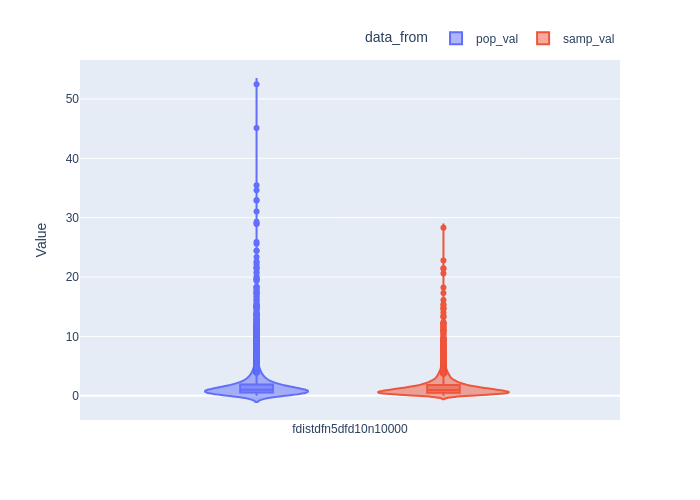
\includegraphics[scale = 0.3]{fdistdfn5dfd10n10000.png}
% }
% \qquad
% \subfigure[F distribution with $=5$, d.f. of denumerator = $15$ and $N=10,000$]{%%\label{}%
%     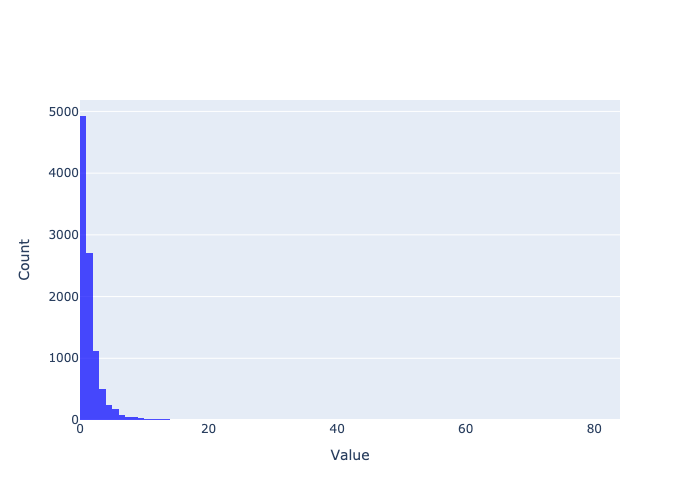
\includegraphics[scale = 0.3]{fdistdfn5dfd15n10000.png}
% }
% \\
% \subfigure[Normal distribution with $mean = 0, \,\,sd = 4$ and $N=10,000$]{%%\label{}%
%     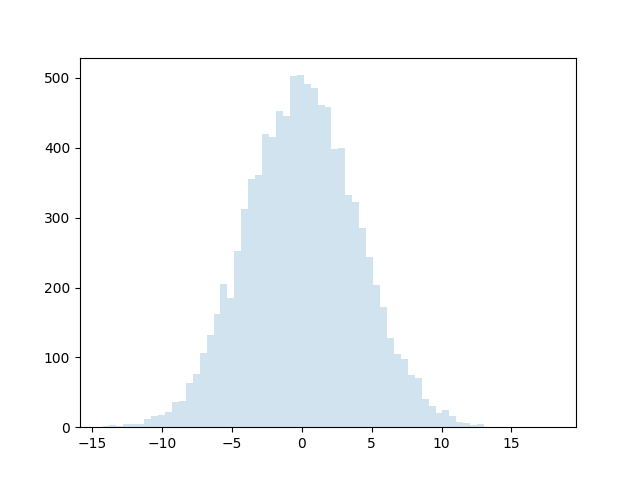
\includegraphics[scale = 0.3]{normalm0sd4n10000.png}
% }
% \qquad
% \subfigure[Normal distribution with $mean = 0, \,\,sd = 1$ and $N=10,000$]{%%\label{}%
%     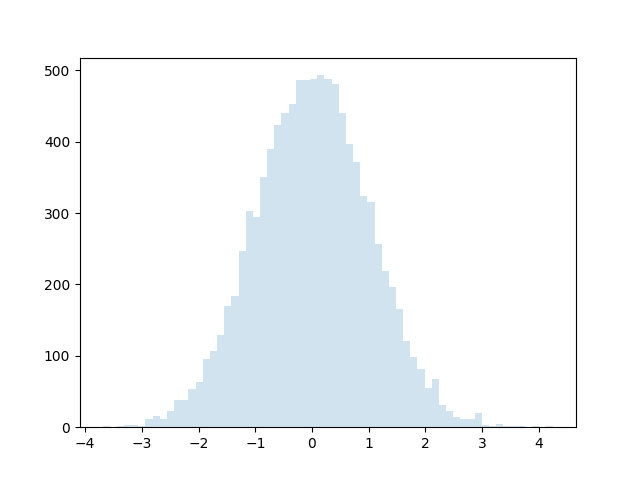
\includegraphics[scale = 0.3]{normalm0sd1n10000.png}
% }
% \\
% \subfigure[Wald distribution with $mean = 1, \,\,sd = 0.5$ and $N=10,000$]{%%\label{}%
%     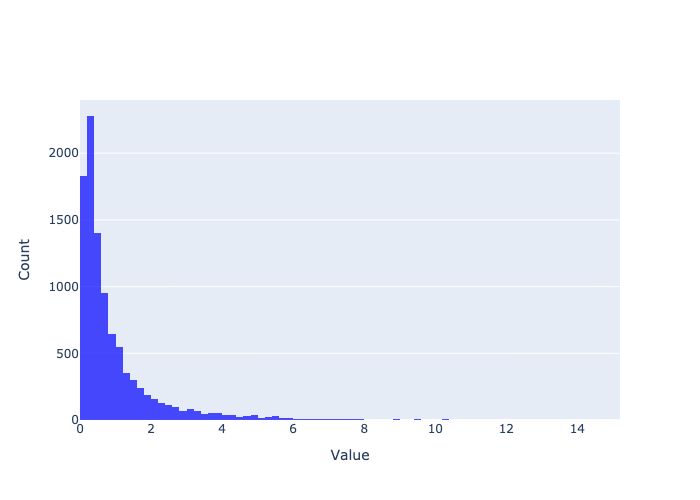
\includegraphics[scale = 0.3]{waldm1sd05n10000.png}
% }
% \qquad
% \subfigure[Wald distribution with $mean = 1, \,\,sd = 2$ and $N=10,000$]{%
% %\label{}%
%     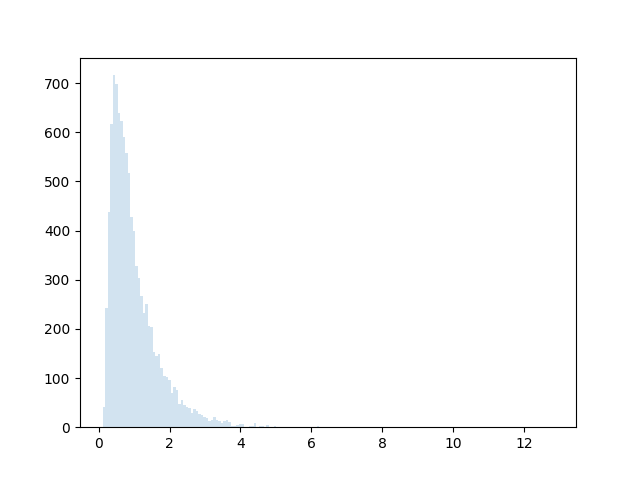
\includegraphics[scale = 0.3]{waldm1sd2n10000.png}
% }
% \\
% \subfigure[Wiebull distribution with $shap = 1$ and $N=10,000$]{%
% %\label{}%
%     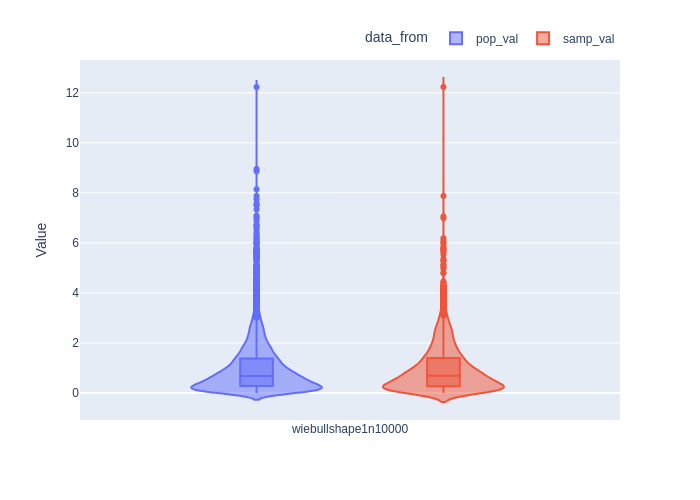
\includegraphics[scale = 0.3]{wiebullshape1n10000.png}
% }
% \qquad
% \subfigure[Wiebull distribution with $shap = 1$ and $N=10,000$]{%
% %\label{}%
%     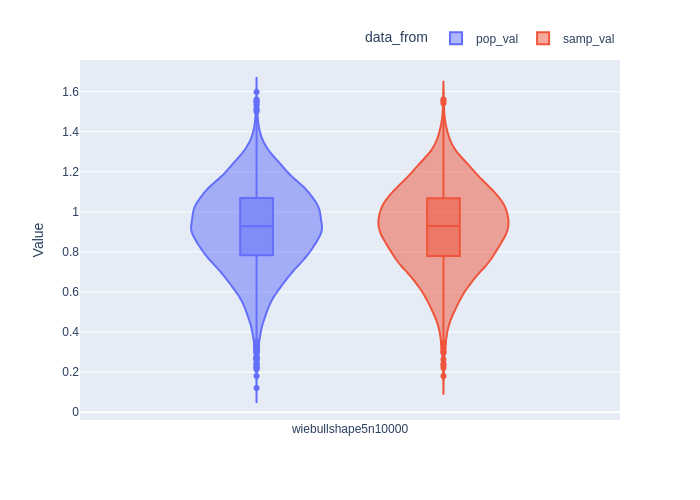
\includegraphics[scale = 0.3]{wiebullshape5n10000.png}
% }
% \caption{Simulated data distribution}\label{Case1:Moder} 
% \end{figure*}

% \begin{figure*}[!t]
% \centering
% \subfigure[laptop prices]{%%\label{}%
%     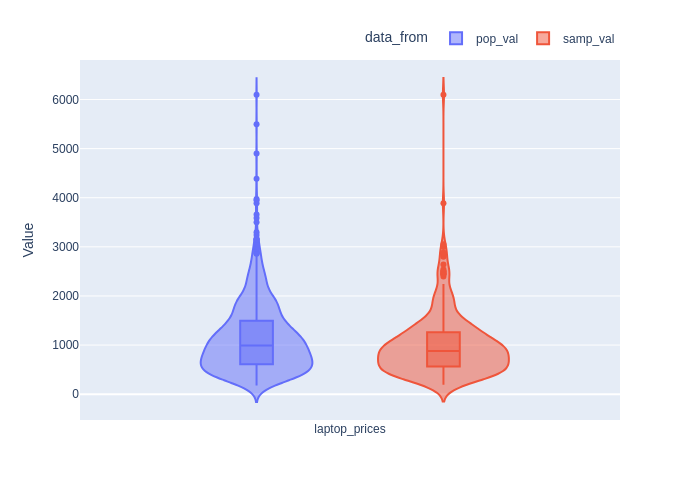
\includegraphics[scale = 0.3]{laptop_prices.png}
% }
% \qquad
% \subfigure[Electronic sales]{%%\label{}%
%     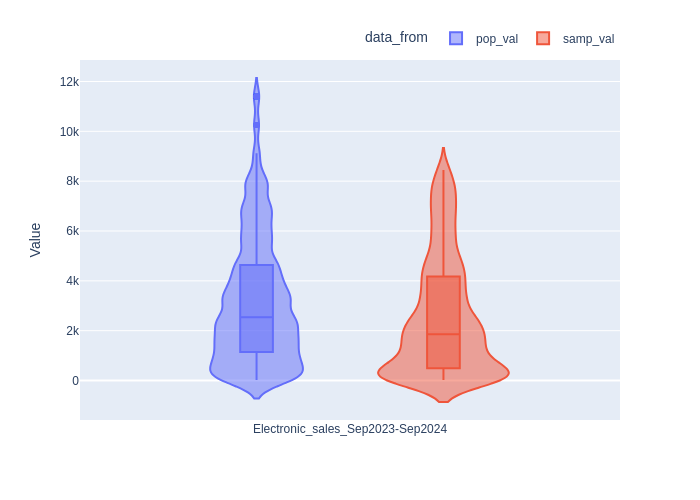
\includegraphics[scale = 0.3]{Electronic_sales_Sep2023-Sep2024.png}
% }
% \\
% \subfigure[Ecommerce sales]{%%\label{}%
%     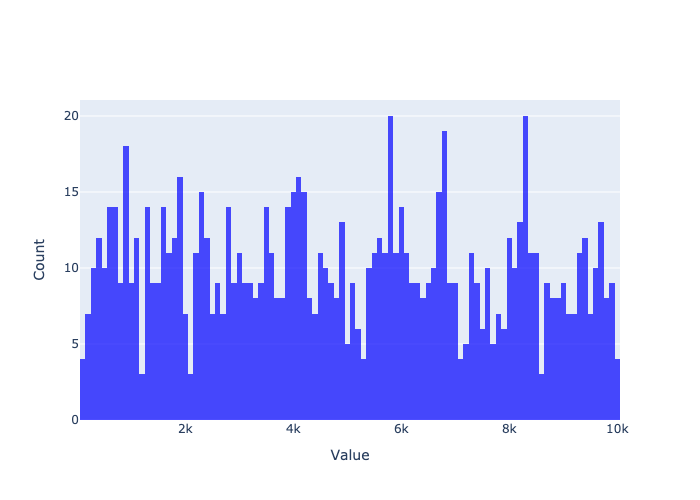
\includegraphics[scale = 0.3]{Ecommerce_Sales_Prediction_Dataset.png}
% }
% \qquad
% \subfigure[world tourism economy data]{%%\label{}%
%     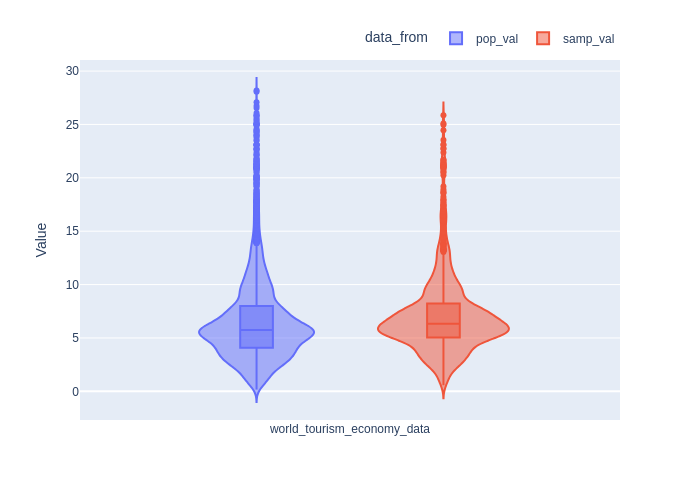
\includegraphics[scale = 0.3]{world_tourism_economy_data.png}
% }
% \caption{real-world data distribution}\label{Case1:Moder} 

% \end{figure*}

%##########
\begin{figure*}[!t]
\centering
\subfigure[]{%
%\label{}%
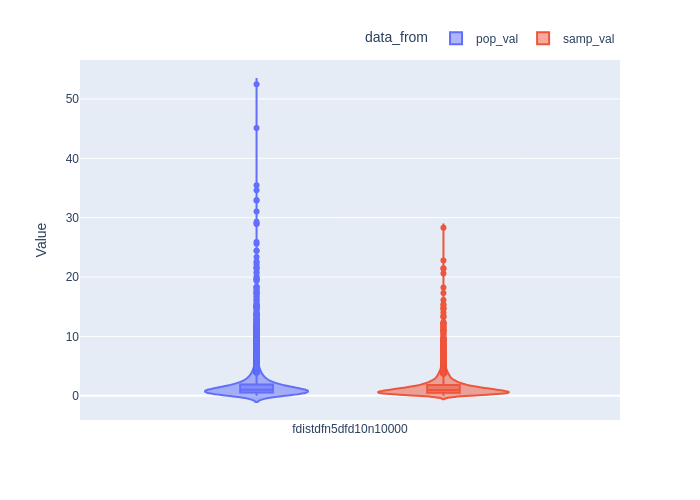
\includegraphics[scale = 0.3]{fdistdfn5dfd10n10000.png}}
\\
\subfigure[]{%
%\label{}%
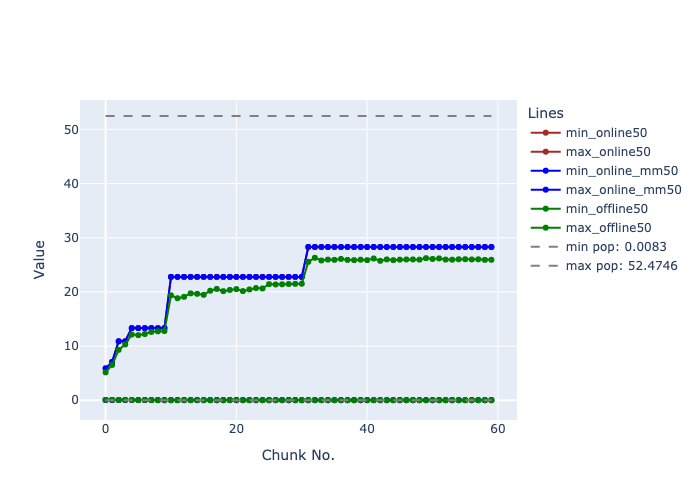
\includegraphics[scale = 0.2]{fdistdfn5dfd10n10000online50.png}}
\qquad
\subfigure[]{%
%\label{}%
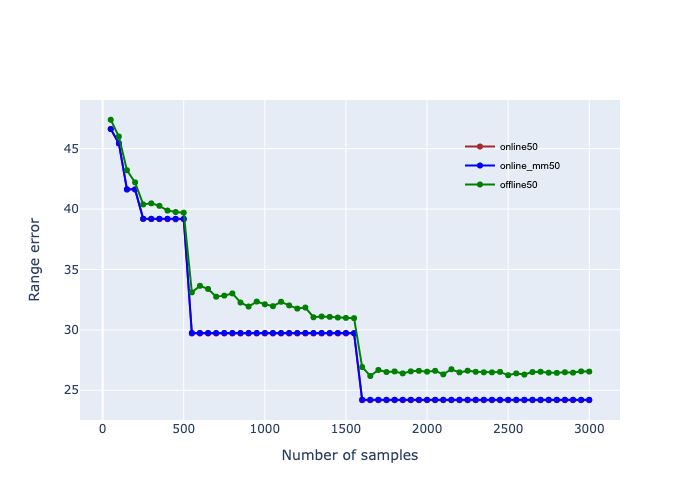
\includegraphics[scale = 0.2]{fdistdfn5dfd10n10000online50error.png}}
\qquad
\subfigure[]{%
%\label{}%
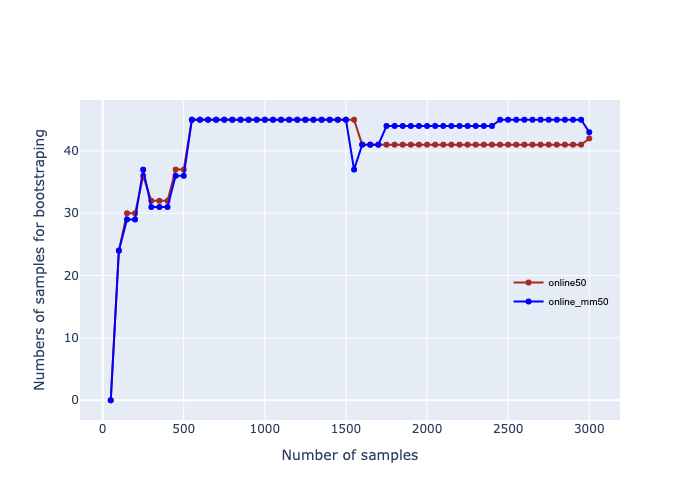
\includegraphics[scale = 0.2]{fdistdfn5dfd10n10000online50_n.png}}
\\
\subfigure[]{%
%\label{}%
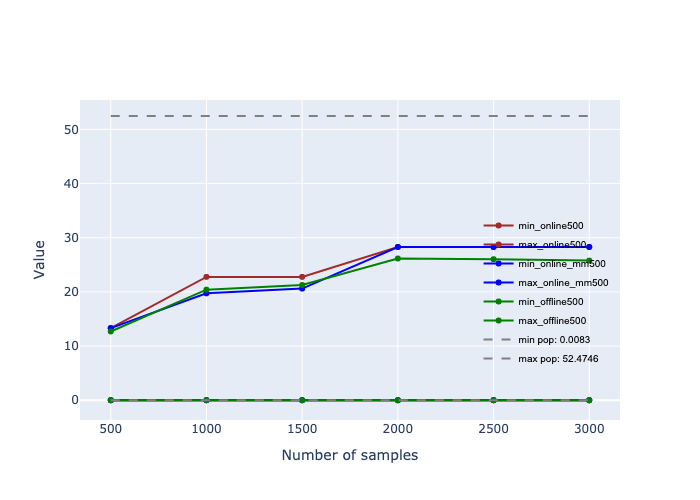
\includegraphics[scale = 0.2]{fdistdfn5dfd10n10000online500.png}}
\qquad
\subfigure[]{%
%\label{}%
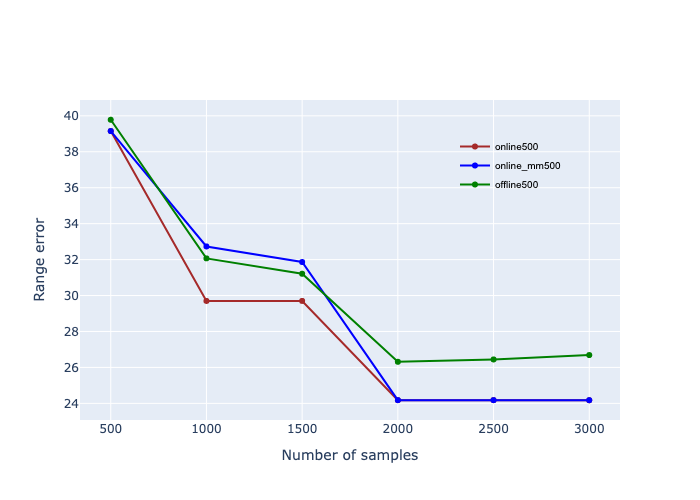
\includegraphics[scale = 0.2]{fdistdfn5dfd10n10000online500error.png}}
\qquad
\subfigure[]{%
%\label{}%
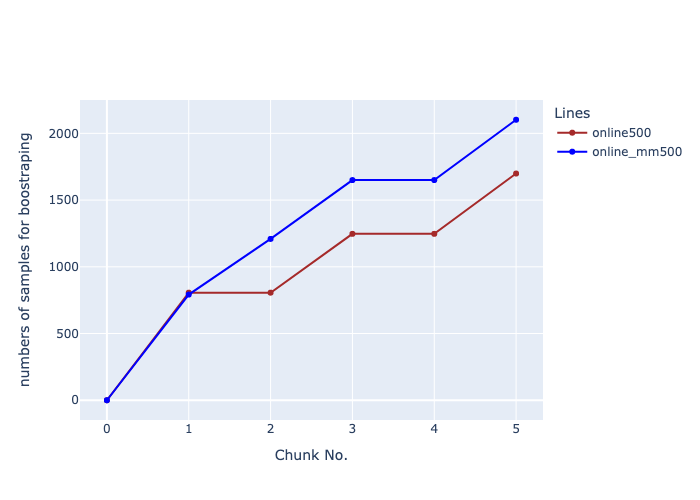
\includegraphics[scale = 0.2]{fdistdfn5dfd10n10000online500_n.png}}
\caption{Range approximation results of $F(\nu_1 =5 ,\nu_2 =10)$ including i) histogram of population data as shown in (a), ii) min-max approximation, range error and number of leftmost and rightmost bins for bootstrapping, for 50 samples/chunk, as shown in (b), (c), and (d), respectively, and iii) min-max approximation, range error and number of leftmost and rightmost bins for bootstrapping, for 500 samples/chunk, as shown in (e), (f), and (g), respectively. }\label{res:fdist1} 
\end{figure*}

\begin{figure*}[!t]
\centering
\subfigure[]{%
%\label{}%
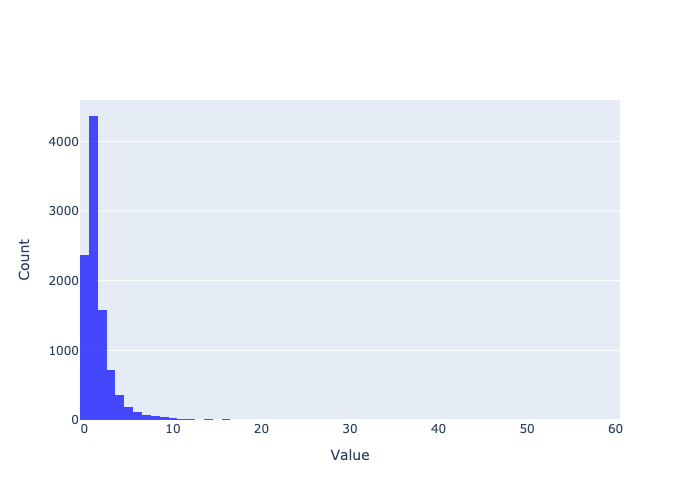
\includegraphics[scale = 0.3]{fdistdfn5dfd20n10000.png}}
\\
\subfigure[]{%
%\label{}%
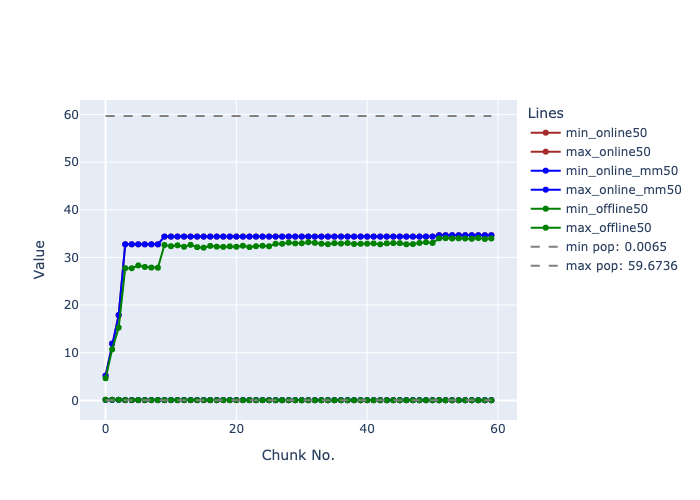
\includegraphics[scale = 0.2]{fdistdfn5dfd20n10000online50.png}}
\qquad
\subfigure[]{%
%\label{}%
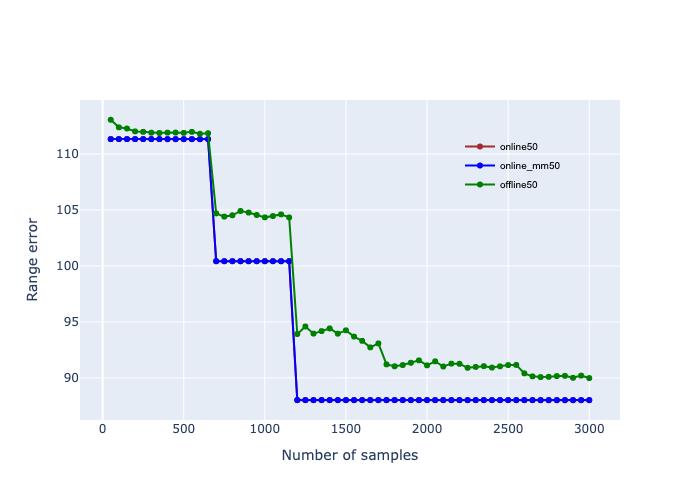
\includegraphics[scale = 0.2]{fdistdfn5dfd20n10000online50error.png}}
\qquad
\subfigure[]{%
%\label{}%
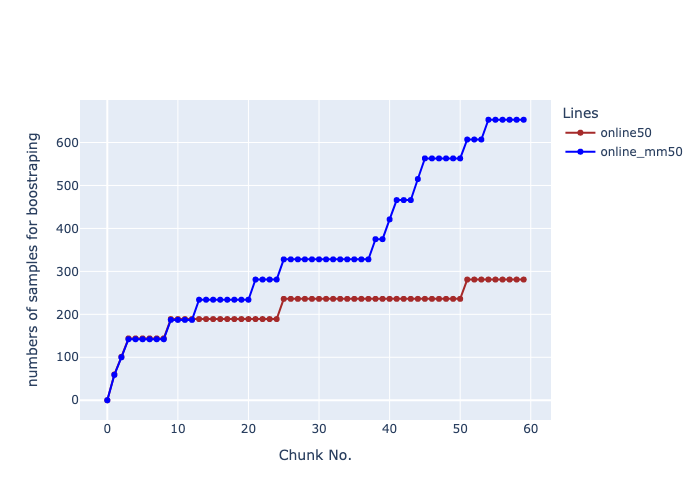
\includegraphics[scale = 0.2]{fdistdfn5dfd20n10000online50_n.png}}
\\
\subfigure[]{%
%\label{}%
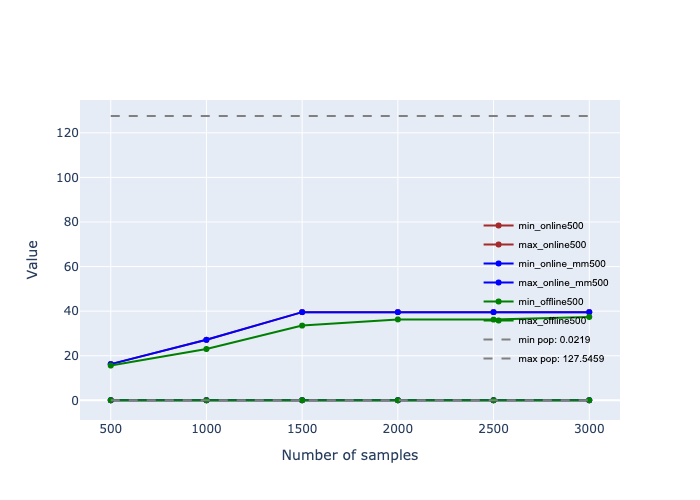
\includegraphics[scale = 0.2]{fdistdfn5dfd20n10000online500.png}}
\qquad
\subfigure[]{%
%\label{}%
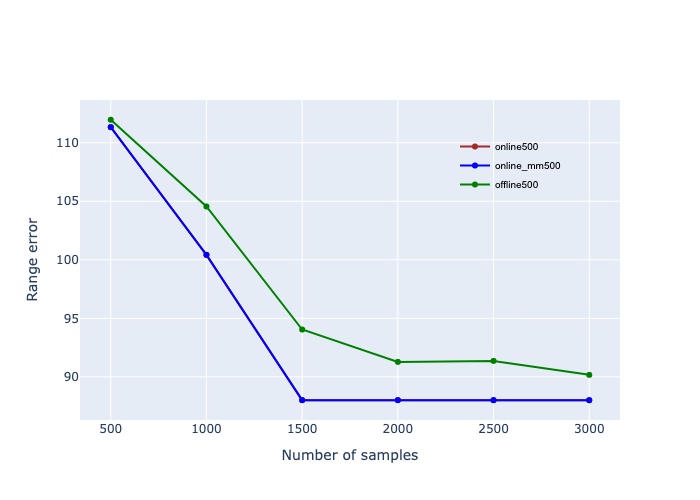
\includegraphics[scale = 0.2]{fdistdfn5dfd20n10000online500error.png}}
\qquad
\subfigure[]{%
%\label{}%
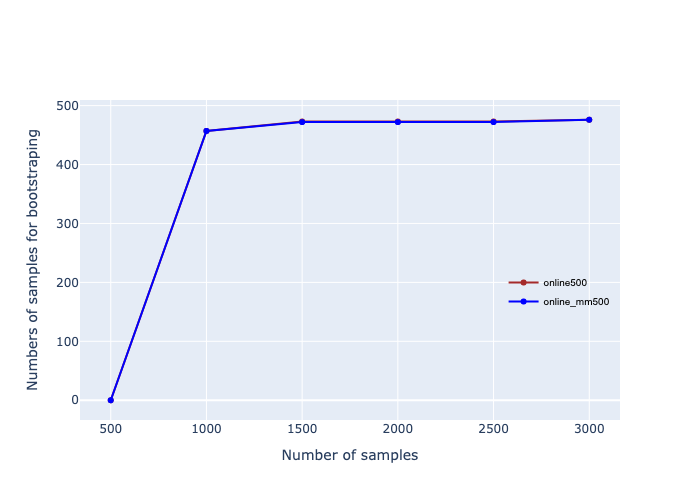
\includegraphics[scale = 0.2]{fdistdfn5dfd20n10000online500_n.png}}
\caption{Range approximation results of $F(\nu_1 =5 ,\nu_2 =20)$ including i) histogram of population data as shown in (a), ii) min-max approximation, range error and number of leftmost and rightmost bins for bootstrapping, for 50 samples/chunk, as shown in (b), (c), and (d), respectively, and iii) min-max approximation, range error and number of leftmost and rightmost bins for bootstrapping, for 500 samples/chunk, as shown in (e), (f), and (g), respectively. }\label{res:fdist2} 
\end{figure*}

\begin{figure*}[!t]
\centering
\subfigure[]{%
%\label{}%
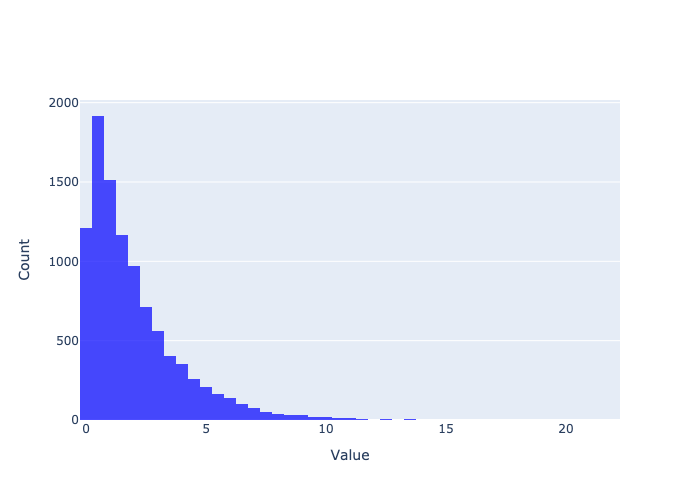
\includegraphics[scale = 0.3]{chi2df2n10000.png}}
\\
\subfigure[]{%
%\label{}%
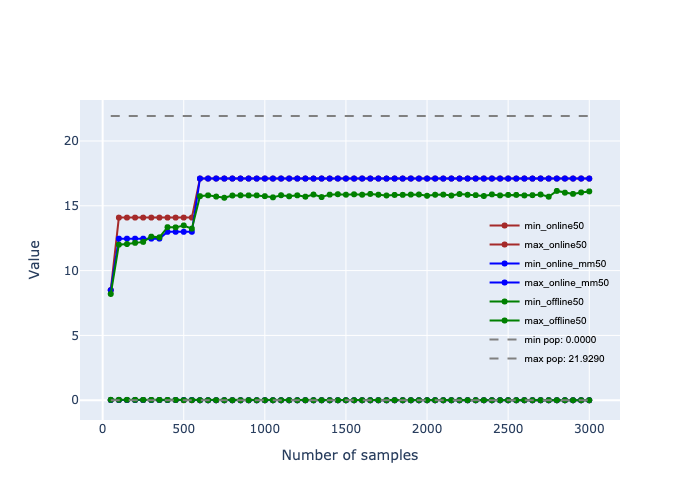
\includegraphics[scale = 0.2]{chi2df2n10000online50.png}}
\qquad
\subfigure[]{%
%\label{}%
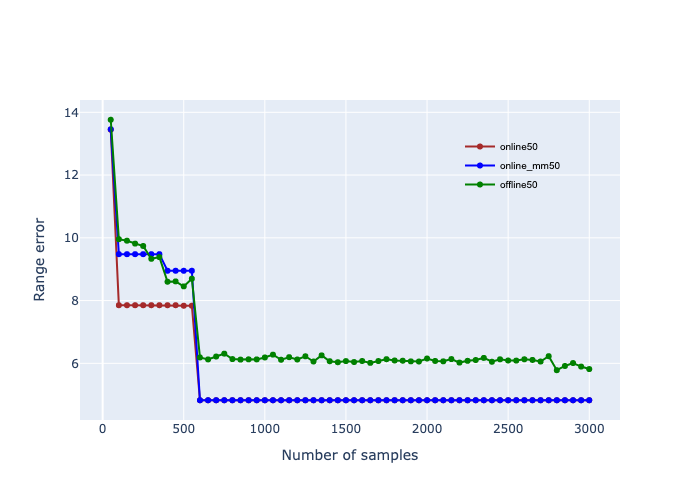
\includegraphics[scale = 0.2]{chi2df2n10000online50error.png}}
\qquad
\subfigure[]{%
%\label{}%
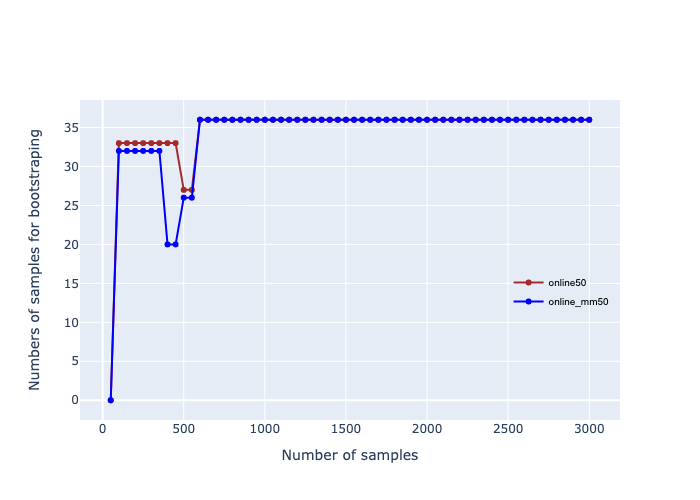
\includegraphics[scale = 0.2]{chi2df2n10000online50_n.png}}
\\
\subfigure[]{%
%\label{}%
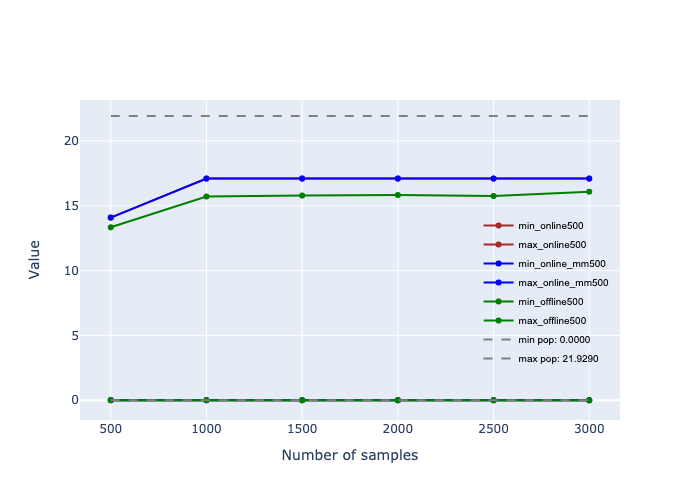
\includegraphics[scale = 0.2]{chi2df2n10000online500.png}}
\qquad
\subfigure[]{%
%\label{}%
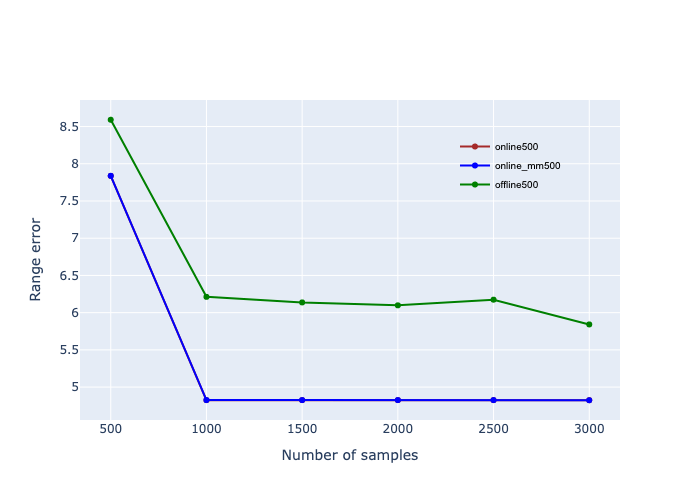
\includegraphics[scale = 0.2]{chi2df2n10000online500error.png}}
\qquad
\subfigure[]{%
%\label{}%
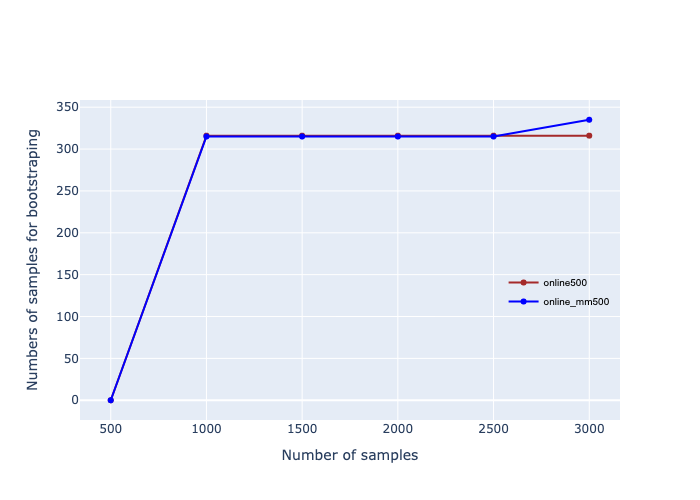
\includegraphics[scale = 0.2]{chi2df2n10000online500_n.png}}
\caption{Range approximation results of $\chi^2(\nu =2)$ including i) histogram of population data as shown in (a), ii) min-max approximation, range error and number of leftmost and rightmost bins for bootstrapping, for 50 samples/chunk, as shown in (b), (c), and (d), respectively, and iii) min-max approximation, range error and number of leftmost and rightmost bins for bootstrapping, for 500 samples/chunk, as shown in (e), (f), and (g), respectively. }\label{res:chidist1} 
\end{figure*}

\begin{figure*}[!t]
\centering
\subfigure[]{%
%\label{}%
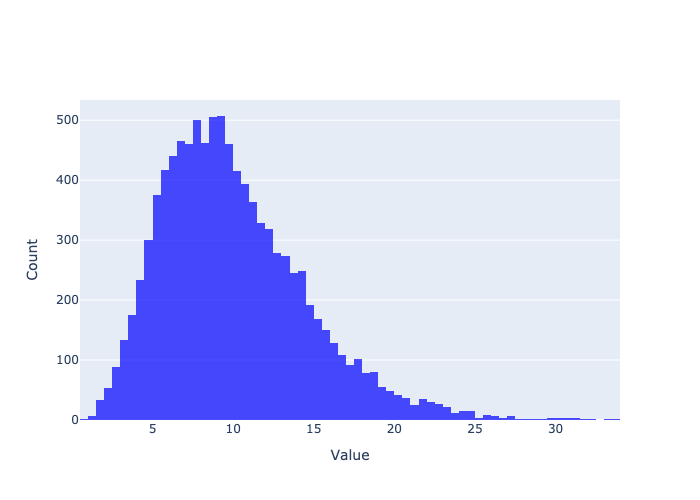
\includegraphics[scale = 0.3]{chi2df10n10000.png}}
\\
\subfigure[]{%
%\label{}%
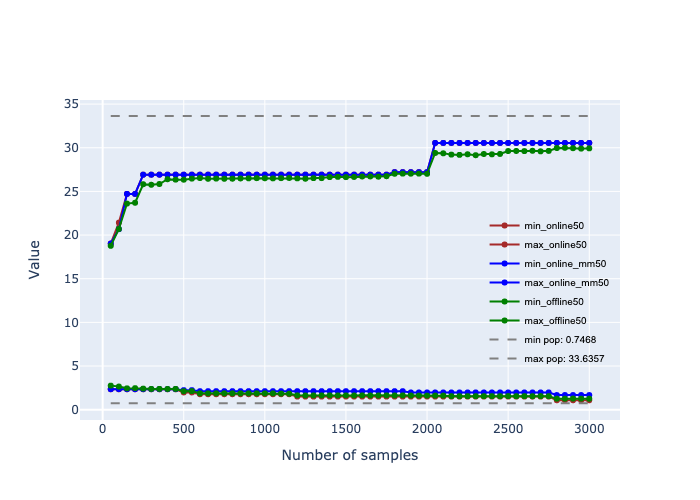
\includegraphics[scale = 0.2]{chi2df10n10000online50.png}}
\qquad
\subfigure[]{%
%\label{}%
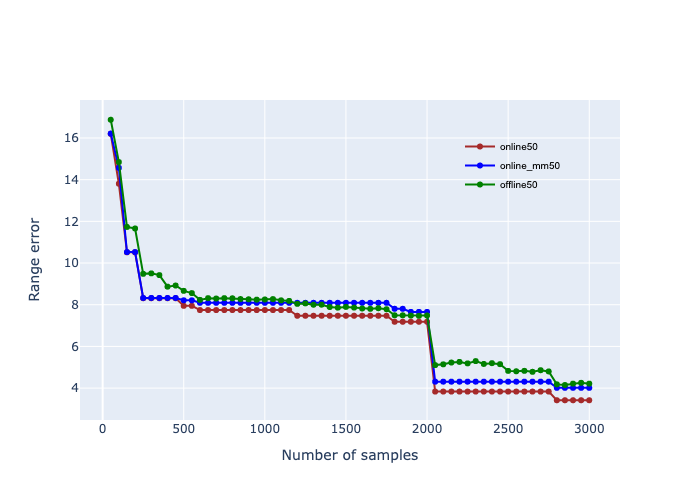
\includegraphics[scale = 0.2]{chi2df10n10000online50error.png}}
\qquad
\subfigure[]{%
%\label{}%
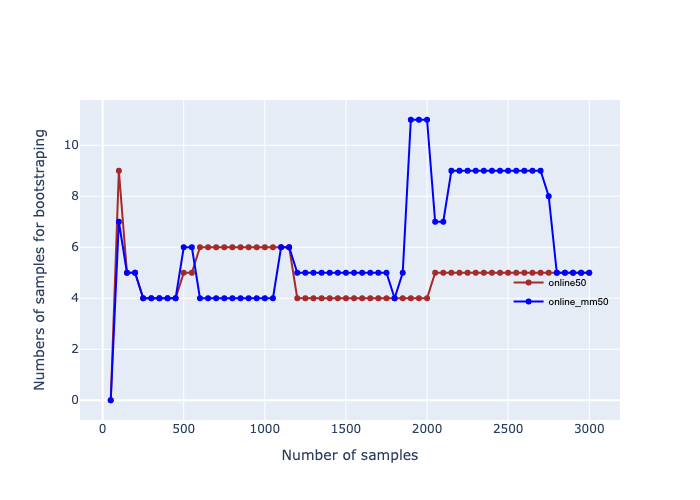
\includegraphics[scale = 0.2]{chi2df10n10000online50_n.png}}
\\
\subfigure[]{%
%\label{}%
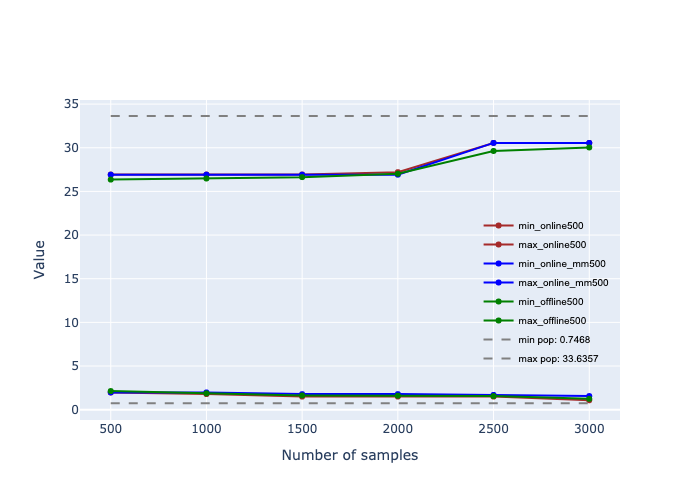
\includegraphics[scale = 0.2]{chi2df10n10000online500.png}}
\qquad
\subfigure[]{%
%\label{}%
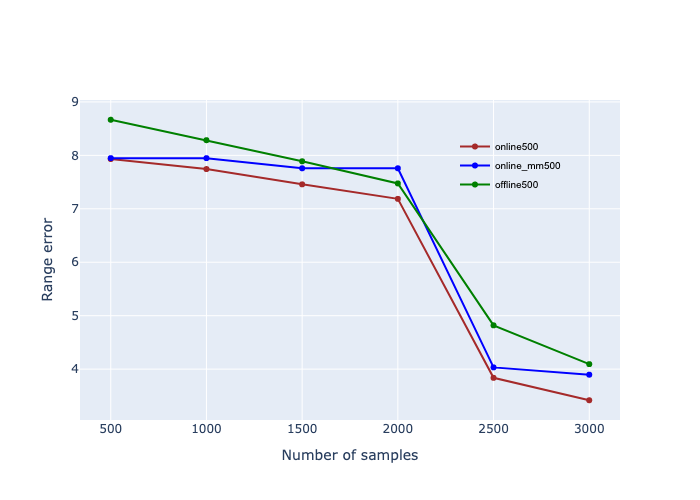
\includegraphics[scale = 0.2]{chi2df10n10000online500error.png}}
\qquad
\subfigure[]{%
%\label{}%
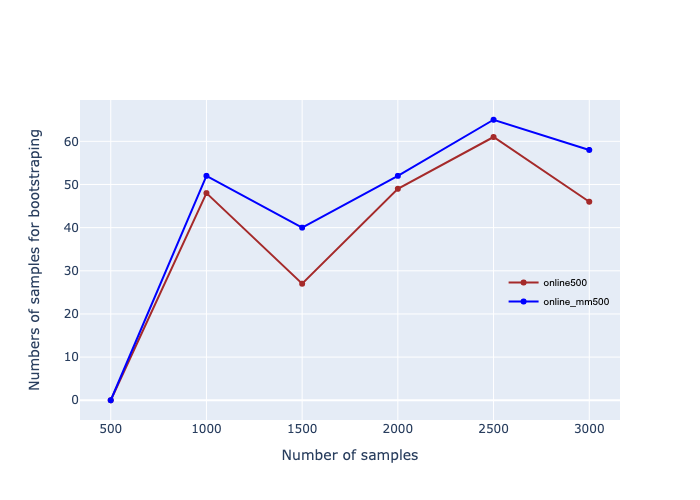
\includegraphics[scale = 0.2]{chi2df10n10000online500_n.png}}
\caption{Range approximation results of $\chi^2(\nu =10)$ including i) histogram of population data as shown in (a), ii) min-max approximation, range error and number of leftmost and rightmost bins for bootstrapping, for 50 samples/chunk, as shown in (b), (c), and (d), respectively, and iii) min-max approximation, range error and number of leftmost and rightmost bins for bootstrapping, for 500 samples/chunk, as shown in (e), (f), and (g), respectively. }\label{res:chidist2} 
\end{figure*}

\begin{figure*}[!t]
\centering
\subfigure[]{%
%\label{}%
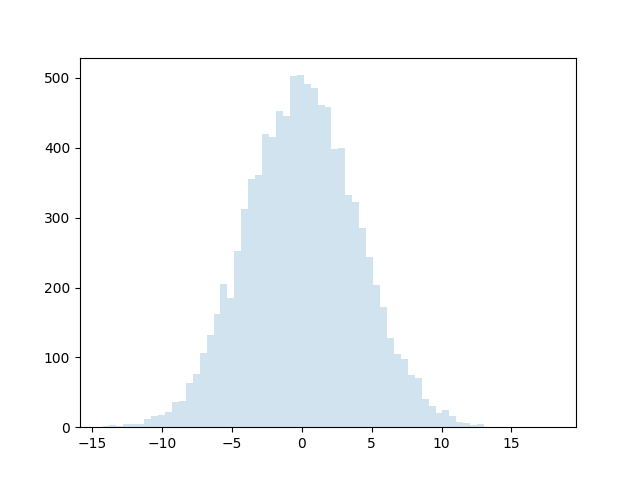
\includegraphics[scale = 0.3]{normalm0sd4n10000.png}}
\\
\subfigure[]{%
%\label{}%
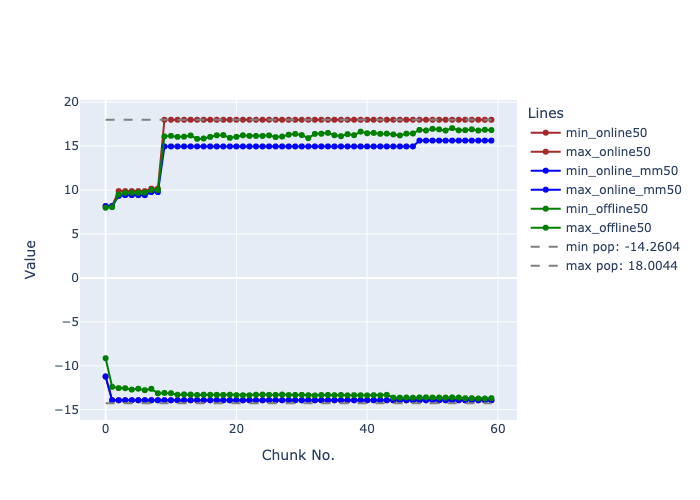
\includegraphics[scale = 0.2]{normalm0sd4n10000online50.png}}
\qquad
\subfigure[]{%
%\label{}%
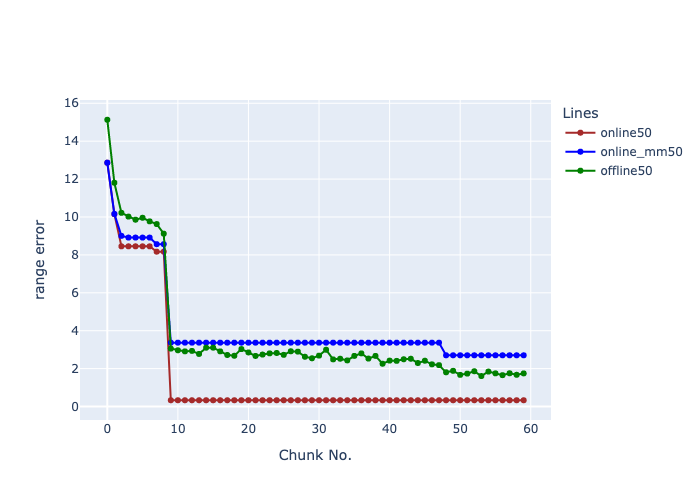
\includegraphics[scale = 0.2]{normalm0sd4n10000online50error.png}}
\qquad
\subfigure[]{%
%\label{}%
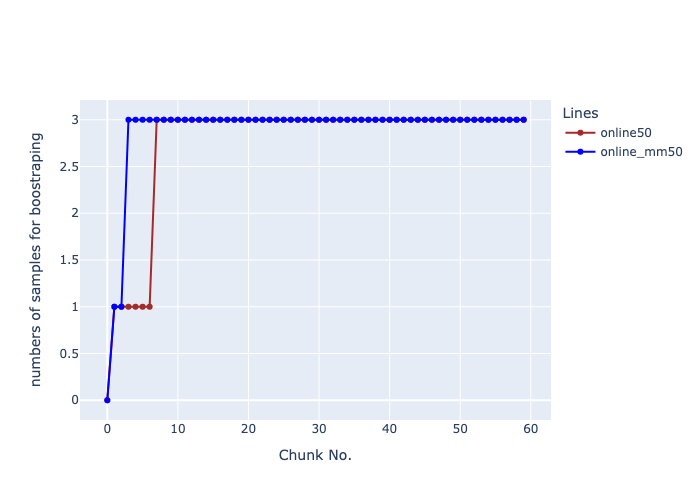
\includegraphics[scale = 0.2]{normalm0sd4n10000online50_n.png}}
\\
\subfigure[]{%
%\label{}%
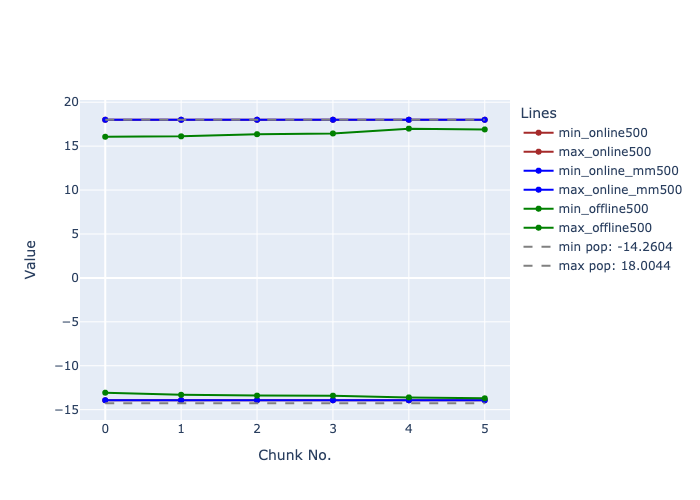
\includegraphics[scale = 0.2]{normalm0sd4n10000online500.png}}
\qquad
\subfigure[]{%
%\label{}%
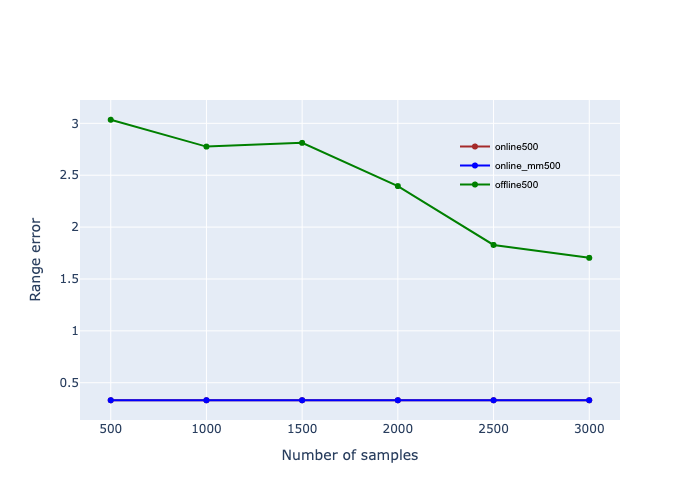
\includegraphics[scale = 0.2]{normalm0sd4n10000online500error.png}}
\qquad
\subfigure[]{%
%\label{}%
\includegraphics[scale = 0.2]{normalm0sd4n10000online500_n.png}}
\caption{Range approximation results of $N(\mu =0 ,\sigma^2 =16)$ including i) histogram of population data as shown in (a), ii) min-max approximation, range error and number of leftmost and rightmost bins for bootstrapping, for 50 samples/chunk, as shown in (b), (c), and (d), respectively, and iii) min-max approximation, range error and number of leftmost and rightmost bins for bootstrapping, for 500 samples/chunk, as shown in (e), (f), and (g), respectively. }\label{res:normaldist1} 
\end{figure*}

\begin{figure*}[!t]
\centering
\subfigure[]{%
%\label{}%
\includegraphics[scale = 0.3]{normalm0sd1n10000.png}}
\\
\subfigure[]{%
%\label{}%
\includegraphics[scale = 0.2]{normalm0sd1n10000online50.png}}
\qquad
\subfigure[]{%
%\label{}%
\includegraphics[scale = 0.2]{normalm0sd1n10000online50error.png}}
\qquad
\subfigure[]{%
%\label{}%
\includegraphics[scale = 0.2]{normalm0sd1n10000online50_n.png}}
\\
\subfigure[]{%
%\label{}%
\includegraphics[scale = 0.2]{normalm0sd1n10000online500.png}}
\qquad
\subfigure[]{%
%\label{}%
\includegraphics[scale = 0.2]{normalm0sd1n10000online500error.png}}
\qquad
\subfigure[]{%
%\label{}%
\includegraphics[scale = 0.2]{normalm0sd1n10000online500_n.png}}
\caption{Range approximation results of $N(\mu =0 ,\sigma^2 =1)$ including i) histogram of population data as shown in (a), ii) min-max approximation, range error and number of leftmost and rightmost bins for bootstrapping, for 50 samples/chunk, as shown in (b), (c), and (d), respectively, and iii) min-max approximation, range error and number of leftmost and rightmost bins for bootstrapping, for 500 samples/chunk, as shown in (e), (f), and (g), respectively. }\label{res:normaldist2} 
\end{figure*}

\begin{figure*}[!t]
\centering
\subfigure[]{%
%\label{}%
\includegraphics[scale = 0.3]{waldm1sd05n10000.png}}
\\
\subfigure[]{%
%\label{}%
\includegraphics[scale = 0.2]{waldm1sd05n10000online50.png}}
\qquad
\subfigure[]{%
%\label{}%
\includegraphics[scale = 0.2]{waldm1sd05n10000online50error.png}}
\qquad
\subfigure[]{%
%\label{}%
\includegraphics[scale = 0.2]{waldm1sd05n10000online50_n.png}}
\\
\subfigure[]{%
%\label{}%
\includegraphics[scale = 0.2]{waldm1sd05n10000online500.png}}
\qquad
\subfigure[]{%
%\label{}%
\includegraphics[scale = 0.2]{waldm1sd05n10000online500error.png}}
\qquad
\subfigure[]{%
%\label{}%
\includegraphics[scale = 0.2]{waldm1sd05n10000online500_n.png}}
\caption{Range approximation results of $Wald(\mu =1 ,\lambda =0.5)$ including i) histogram of population data as shown in (a), ii) min-max approximation, range error and number of leftmost and rightmost bins for bootstrapping, for 50 samples/chunk, as shown in (b), (c), and (d), respectively, and iii) min-max approximation, range error and number of leftmost and rightmost bins for bootstrapping, for 500 samples/chunk, as shown in (e), (f), and (g), respectively. }\label{res:walddist1} 
\end{figure*}

\begin{figure*}[!t]
\centering
\subfigure[]{%
%\label{}%
\includegraphics[scale = 0.3]{waldm1sd2n10000.png}}
\\
\subfigure[]{%
%\label{}%
\includegraphics[scale = 0.2]{waldm1sd2n10000online50.png}}
\qquad
\subfigure[]{%
%\label{}%
\includegraphics[scale = 0.2]{waldm1sd2n10000online50error.png}}
\qquad
\subfigure[]{%
%\label{}%
\includegraphics[scale = 0.2]{waldm1sd2n10000online50_n.png}}
\\
\subfigure[]{%
%\label{}%
\includegraphics[scale = 0.2]{waldm1sd2n10000online500.png}}
\qquad
\subfigure[]{%
%\label{}%
\includegraphics[scale = 0.2]{waldm1sd2n10000online500error.png}}
\qquad
\subfigure[]{%
%\label{}%
\includegraphics[scale = 0.2]{waldm1sd2n10000online500_n.png}}
\caption{Range approximation results of $Wald(\mu =1 ,\lambda =2.0)$ including i) histogram of population data as shown in (a), ii) min-max approximation, range error and number of leftmost and rightmost bins for bootstrapping, for 50 samples/chunk, as shown in (b), (c), and (d), respectively, and iii) min-max approximation, range error and number of leftmost and rightmost bins for bootstrapping, for 500 samples/chunk, as shown in (e), (f), and (g), respectively. }\label{res:walddist2} 
\end{figure*}

\begin{figure*}[!t]
\centering
\subfigure[]{%
%\label{}%
\includegraphics[scale = 0.3]{wiebullshape1n10000.png}}
\\
\subfigure[]{%
%\label{}%
\includegraphics[scale = 0.2]{wiebullshape1n10000online50.png}}
\qquad
\subfigure[]{%
%\label{}%
\includegraphics[scale = 0.2]{wiebullshape1n10000online50error.png}}
\qquad
\subfigure[]{%
%\label{}%
\includegraphics[scale = 0.2]{wiebullshape1n10000online50_n.png}}
\\
\subfigure[]{%
%\label{}%
\includegraphics[scale = 0.2]{wiebullshape1n10000online500.png}}
\qquad
\subfigure[]{%
%\label{}%
\includegraphics[scale = 0.2]{wiebullshape1n10000online500error.png}}
\qquad
\subfigure[]{%
%\label{}%
\includegraphics[scale = 0.2]{wiebullshape1n10000online500_n.png}}
\caption{Range approximation results of $Weibull(shape =1)$ including i) histogram of population data as shown in (a), ii) min-max approximation, range error and number of leftmost and rightmost bins for bootstrapping, for 50 samples/chunk, as shown in (b), (c), and (d), respectively, and iii) min-max approximation, range error and number of leftmost and rightmost bins for bootstrapping, for 500 samples/chunk, as shown in (e), (f), and (g), respectively. }\label{res:weibulldist1} 
\end{figure*}

\begin{figure*}[!t]
\centering
\subfigure[]{%
%\label{}%
\includegraphics[scale = 0.3]{wiebullshape5n10000.png}}
\\
\subfigure[]{%
%\label{}%
\includegraphics[scale = 0.2]{wiebullshape5n10000online50.png}}
\qquad
\subfigure[]{%
%\label{}%
\includegraphics[scale = 0.2]{wiebullshape5n10000online50error.png}}
\qquad
\subfigure[]{%
%\label{}%
\includegraphics[scale = 0.2]{wiebullshape5n10000online50_n.png}}
\\
\subfigure[]{%
%\label{}%
\includegraphics[scale = 0.2]{wiebullshape5n10000online500.png}}
\qquad
\subfigure[]{%
%\label{}%
\includegraphics[scale = 0.2]{wiebullshape5n10000online500error.png}}
\qquad
\subfigure[]{%
%\label{}%
\includegraphics[scale = 0.2]{wiebullshape5n10000online500_n.png}}
\caption{Range approximation results of $Weibull(shape =5)$ including i) histogram of population data as shown in (a), ii) min-max approximation, range error and number of leftmost and rightmost bins for bootstrapping, for 50 samples/chunk, as shown in (b), (c), and (d), respectively, and iii) min-max approximation, range error and number of leftmost and rightmost bins for bootstrapping, for 500 samples/chunk, as shown in (e), (f), and (g), respectively. }\label{res:weibulldist2} 
\end{figure*}

% Realworld cases 
\begin{figure*}[!t]
\centering
\subfigure[]{%
%\label{}%
\includegraphics[scale = 0.3]{laptop_prices.png}}
\\
\subfigure[]{%
%\label{}%
\includegraphics[scale = 0.2]{laptop_pricesonline50.png}}
\qquad
\subfigure[]{%
%\label{}%
\includegraphics[scale = 0.2]{laptop_pricesonline50error.png}}
\qquad
\subfigure[]{%
%\label{}%
\includegraphics[scale = 0.2]{laptop_pricesonline50error.png}}
\\
\subfigure[]{%
%\label{}%
\includegraphics[scale = 0.2]{laptop_pricesonline100.png}}
\qquad
\subfigure[]{%
%\label{}%
\includegraphics[scale = 0.2]{laptop_pricesonline100error.png}}
\qquad
\subfigure[]{%
%\label{}%
\includegraphics[scale = 0.2]{laptop_pricesonline100_n.png}}
\caption{Range approximation results of laptop prices including i) histogram of population data as shown in (a), ii) min-max approximation, range error and number of leftmost and rightmost bins for bootstrapping, for 50 samples/chunk, as shown in (b), (c), and (d), respectively, and iii) min-max approximation, range error and number of leftmost and rightmost bins for bootstrapping, for 500 samples/chunk, as shown in (e), (f), and (g), respectively. }\label{res:laptop} 
\end{figure*}

\begin{figure*}[!t]
\centering
\subfigure[]{%
%\label{}%
\includegraphics[scale = 0.3]{Electronic_sales_Sep2023-Sep2024.png}}
\\
\subfigure[]{%
%\label{}%
\includegraphics[scale = 0.2]{Electronic_sales_Sep2023-Sep2024online50.png}}
\qquad
\subfigure[]{%
%\label{}%
\includegraphics[scale = 0.2]{Electronic_sales_Sep2023-Sep2024online50error.png}}
\qquad
\subfigure[]{%
%\label{}%
\includegraphics[scale = 0.2]{Electronic_sales_Sep2023-Sep2024online50_n.png}}
\\
\subfigure[]{%
%\label{}%
\includegraphics[scale = 0.2]{Electronic_sales_Sep2023-Sep2024online100.png}}
\qquad
\subfigure[]{%
%\label{}%
\includegraphics[scale = 0.2]{Electronic_sales_Sep2023-Sep2024online100error.png}}
\qquad
\subfigure[]{%
%\label{}%
\includegraphics[scale = 0.2]{Electronic_sales_Sep2023-Sep2024online100error.png}}
\caption{Range approximation results of Electronic sales including i) histogram of population data as shown in (a), ii) min-max approximation, range error and number of leftmost and rightmost bins for bootstrapping, for 50 samples/chunk, as shown in (b), (c), and (d), respectively, and iii) min-max approximation, range error and number of leftmost and rightmost bins for bootstrapping, for 500 samples/chunk, as shown in (e), (f), and (g), respectively. }\label{res:elect} 
\end{figure*}

\begin{figure*}[!t]
\centering
\subfigure[]{%
%\label{}%
\includegraphics[scale = 0.3]{Ecommerce_Sales_Prediction_Dataset.png}}
\\
\subfigure[]{%
%\label{}%
\includegraphics[scale = 0.2]{Ecommerce_Sales_Prediction_Datasetonline50.png}}
\qquad
\subfigure[]{%
%\label{}%
\includegraphics[scale = 0.2]{Ecommerce_Sales_Prediction_Datasetonline50error.png}}
\qquad
\subfigure[]{%
%\label{}%
\includegraphics[scale = 0.2]{Ecommerce_Sales_Prediction_Datasetonline50error.png}}
\\
\subfigure[]{%
%\label{}%
\includegraphics[scale = 0.2]{Ecommerce_Sales_Prediction_Datasetonline100.png}}
\qquad
\subfigure[]{%
%\label{}%
\includegraphics[scale = 0.2]{Ecommerce_Sales_Prediction_Datasetonline100error.png}}
\qquad
\subfigure[]{%
%\label{}%
\includegraphics[scale = 0.2]{Ecommerce_Sales_Prediction_Datasetonline100_n.png}}
\caption{Range approximation results of e-commerce sales including i) histogram of population data as shown in (a), ii) min-max approximation, range error and number of leftmost and rightmost bins for bootstrapping, for 50 samples/chunk, as shown in (b), (c), and (d), respectively, and iii) min-max approximation, range error and number of leftmost and rightmost bins for bootstrapping, for 500 samples/chunk, as shown in (e), (f), and (g), respectively. }\label{res:ecom} 
\end{figure*}

\begin{figure*}[!t]
\centering
\subfigure[]{%
%\label{}%
\includegraphics[scale = 0.3]{world_tourism_economy_data.png}}
\\
\subfigure[]{%
%\label{}%
\includegraphics[scale = 0.2]{world_tourism_economy_dataonline50.png}}
\qquad
\subfigure[]{%
%\label{}%
\includegraphics[scale = 0.2]{world_tourism_economy_dataonline50error.png}}
\qquad
\subfigure[]{%
%\label{}%
\includegraphics[scale = 0.2]{world_tourism_economy_dataonline50_n.png}}
\\
\subfigure[]{%
%\label{}%
\includegraphics[scale = 0.2]{world_tourism_economy_dataonline100.png}}
\qquad
\subfigure[]{%
%\label{}%
\includegraphics[scale = 0.2]{world_tourism_economy_dataonline100error.png}}
\qquad
\subfigure[]{%
%\label{}%
\includegraphics[scale = 0.2]{world_tourism_economy_dataonline100_n.png}}
\caption{Range approximation results of world tourism economy including i) histogram of population data as shown in (a), ii) min-max approximation, range error and number of leftmost and rightmost bins for bootstrapping, for 50 samples/chunk, as shown in (b), (c), and (d), respectively, and iii) min-max approximation, range error and number of leftmost and rightmost bins for bootstrapping, for 500 samples/chunk, as shown in (e), (f), and (g), respectively. }\label{res:world} 
\end{figure*}

% \begin{figure*}[!t]
% \centering
% \subfigure[min-max approximation with 50 samples/chunk out of 3,000 samples]{%
% %\label{}%
%     \includegraphics[scale = 0.3]{waldm1sd05n10000online50.png}
% }
% \qquad
% \subfigure[range approximation along the streaming chunks with 50 samples/chunk]{%
% %\label{}%
%     \includegraphics[scale = 0.3]{waldm1sd05n10000online50error.png}
% }
% \\
% \subfigure[min-max approximation with 500 samples/chunks out of 3,000 samples]{%
% %\label{}%
%     \includegraphics[scale = 0.3]{waldm1sd05n10000online500.png}
% }
% \qquad
% \subfigure[range approximation along the streaming chunks with 500 samples/chunk]{%
% %\label{}%
%     \includegraphics[scale = 0.3]{waldm1sd05n10000online500error.png}
% }
% \\
% \subfigure[Number of samples for bootstrapping along the streaming chunks with 50 samples/chunk]{%
% %\label{}%
%     \includegraphics[scale = 0.3]{waldm1sd05n10000online50_n.png}
% }
% \qquad
% \subfigure[Number of samples for bootstrapping along the streaming chunks with 500 samples/chunk]{%
% %\label{}%
%     \includegraphics[scale = 0.3]{waldm1sd05n10000online500_n.png}
% }
% \caption{range approximation of Wald distribution with $mean = 1$, $sd=0.5$ and $N=10,000$}\label{res:wald} 
% \end{figure*}
 


% \begin{figure*}[!t]
% \centering
% \subfigure[min-max approximation with 50 samples/chunk out of 3,000 samples]{%
% %\label{}%
% \includegraphics[scale = 0.3]{waldm1sd2n10000online50.png}}
% \qquad
% \subfigure[range approximation along the streaming chunks with 50 samples/chunk]{%
% %\label{}%
% \includegraphics[scale = 0.3]{waldm1sd2n10000online50error.png}}\\
% \subfigure[min-max approximation with 500 samples/chunks out of 3,000 samples]{%
% %\label{}%
% \includegraphics[scale = 0.3]{waldm1sd2n10000online500.png}}
% \qquad
% \subfigure[range approximation along the streaming chunks with 500 samples/chunk]{%
% %\label{}%
% \includegraphics[scale = 0.3]{waldm1sd2n10000online500error.png}}\\
% \subfigure[Number of samples for bootstrapping along the streaming chunks with 50 samples/chunk]{%
% %\label{}%
% \includegraphics[scale = 0.3]{waldm1sd2n10000online50_n.png}}
% \qquad
% \subfigure[Number of samples for bootstrapping along the streaming chunks with 500 samples/chunk]{%
% %\label{}%
% \includegraphics[scale = 0.3]{waldm1sd2n10000online500_n.png}}
% \caption{range approximation of Wald distribution with $mean = 1$, $sd=2$ and $N=10,000$}\label{res:wald} 
% \end{figure*}



% \begin{figure*}[!t]
% \centering
% % \subfigure[Histogram for Wiebull distribution with $shap = 1$ and $N=10,000$]{%
% % %\label{}%
% % \includegraphics[scale = 0.3]{wiebullshape1n10000.png}}\\
% \subfigure[min-max approximation with 50 samples/chunk out of 3,000 samples]{%
% %\label{}%
% \includegraphics[scale = 0.3]{wiebullshape1n10000online50.png}}
% \qquad
% \subfigure[range approximation along the streaming chunks with 50 samples/chunk]{%
% %\label{}%
% \includegraphics[scale = 0.3]{wiebullshape1n10000online50error.png}}\\
% \subfigure[min-max approximation with 500 samples/chunks out of 3,000 samples]{%
% %\label{}%
% \includegraphics[scale = 0.3]{wiebullshape1n10000online500.png}}
% \qquad
% \subfigure[range approximation along the streaming chunks with 500 samples/chunk]{%
% %\label{}%
% \includegraphics[scale = 0.3]{wiebullshape1n10000online500error.png}}\\
% \subfigure[Number of samples for bootstrapping along the streaming chunks with 50 samples/chunk]{%
% %\label{}%
% \includegraphics[scale = 0.3]{wiebullshape1n10000online50_n.png}}
% \qquad
% \subfigure[Number of samples for bootstrapping along the streaming chunks with 500 samples/chunk]{%
% %\label{}%
% \includegraphics[scale = 0.3]{wiebullshape1n10000online500_n.png}}
% \caption{range approximation of Wiebull distribution with $shap = 1$ and $N=10,000$}\label{Case1:Moder} 
% \end{figure*}

% \begin{figure*}[!t]
% \centering
% % \subfigure[Histogram for Wiebull distribution with $shap = 5$ and $N=10,000$]{%
% % %\label{}%
% % \includegraphics[scale = 0.3]{wiebullshape5n10000.png}}\\
% \subfigure[min-max approximation with 50 samples/chunk out of 3,000 samples]{%
% %\label{}%
% \includegraphics[scale = 0.3]{wiebullshape5n10000online50.png}}
% \qquad
% \subfigure[range approximation along the streaming chunks with 50 samples/chunk]{%
% %\label{}%
% \includegraphics[scale = 0.3]{wiebullshape5n10000online50error.png}}\\
% \subfigure[min-max approximation with 500 samples/chunks out of 3,000 samples]{%
% %\label{}%
% \includegraphics[scale = 0.3]{wiebullshape5n10000online500.png}}
% \qquad
% \subfigure[range approximation along the streaming chunks with 500 samples/chunk]{%
% %\label{}%
% \includegraphics[scale = 0.3]{wiebullshape5n10000online500error.png}}\\
% \subfigure[Number of samples for bootstrapping along the streaming chunks with 50 samples/chunk]{%
% %\label{}%
% \includegraphics[scale = 0.3]{wiebullshape5n10000online50_n.png}}
% \qquad
% \subfigure[Number of samples for bootstrapping along the streaming chunks with 500 samples/chunk]{%
% %\label{}%
% \includegraphics[scale = 0.3]{wiebullshape5n10000online500_n.png}}
% \caption{range approximation of Wiebull distribution with $shap = 5$ and $N=10,000$}\label{Case1:Moder} 
% \end{figure*}

% \begin{figure*}[!t]
% \centering
% \subfigure[min-max approximation with 50 samples/chunk out of 3,000 samples]{%
% %\label{}%
% \includegraphics[scale = 0.3]{laptop_pricesonline50.png}}
% \qquad
% \subfigure[range approximation along the streaming chunks with 50 samples/chunk]{%
% %\label{}%
% \includegraphics[scale = 0.3]{laptop_pricesonline50error.png}}\\
% \subfigure[min-max approximation with 100 samples/chunks out of 3,000 samples]{%
% %\label{}%
% \includegraphics[scale = 0.3]{laptop_pricesonline100.png}}
% \qquad
% \subfigure[range approximation along the streaming chunks with 100 samples/chunk]{%
% %\label{}%
% \includegraphics[scale = 0.3]{laptop_pricesonline100error.png}}\\
% \subfigure[Number of samples for bootstrapping along the streaming chunks with 50 samples/chunk]{%
% %\label{}%
% \includegraphics[scale = 0.3]{laptop_pricesonline50_n.png}}
% \qquad
% \subfigure[Number of samples for bootstrapping along the streaming chunks with 100 samples/chunk]{%
% %\label{}%
% \includegraphics[scale = 0.3]{laptop_pricesonline100_n.png}}
% \caption{range approximation of laptop price data set}\label{res:wald} 
% \end{figure*}

% \begin{figure*}[!t]
% \centering
% \subfigure[min-max approximation with 50 samples/chunk out of 3,000 samples]{%
% %\label{}%
% \includegraphics[scale = 0.3]{Electronic_sales_Sep2023-Sep2024online50.png}}
% \qquad
% \subfigure[range approximation along the streaming chunks with 50 samples/chunk]{%
% %\label{}%
% \includegraphics[scale = 0.3]{Electronic_sales_Sep2023-Sep2024online50error.png}}\\
% \subfigure[min-max approximation with 100 samples/chunks out of 3,000 samples]{%
% %\label{}%
% \includegraphics[scale = 0.3]{Electronic_sales_Sep2023-Sep2024online100.png}}
% \qquad
% \subfigure[range approximation along the streaming chunks with 100 samples/chunk]{%
% %\label{}%
% \includegraphics[scale = 0.3]{Electronic_sales_Sep2023-Sep2024online100error.png}}\\
% \subfigure[Number of samples for bootstrapping along the streaming chunks with 50 samples/chunk]{%
% %\label{}%
% \includegraphics[scale = 0.3]{Electronic_sales_Sep2023-Sep2024online50_n.png}}
% \qquad
% \subfigure[Number of samples for bootstrapping along the streaming chunks with 100 samples/chunk]{%
% %\label{}%
% \includegraphics[scale = 0.3]{Electronic_sales_Sep2023-Sep2024online100_n.png}}
% \caption{range approximation of Electronic sales data set}\label{res:wald} 
% \end{figure*}

% \begin{figure*}[!t]
% \centering
% \subfigure[min-max approximation with 50 samples/chunk out of 3,000 samples]{%
% %\label{}%
% \includegraphics[scale = 0.3]{Ecommerce_Sales_Prediction_Datasetonline50.png}}
% \qquad
% \subfigure[range approximation along the streaming chunks with 50 samples/chunk]{%
% %\label{}%
% \includegraphics[scale = 0.3]{Ecommerce_Sales_Prediction_Datasetonline50error.png}}\\
% \subfigure[min-max approximation with 100 samples/chunks out of 3,000 samples]{%
% %\label{}%
% \includegraphics[scale = 0.3]{Ecommerce_Sales_Prediction_Datasetonline100.png}}
% \qquad
% \subfigure[range approximation along the streaming chunks with 100 samples/chunk]{%
% %\label{}%
% \includegraphics[scale = 0.3]{Ecommerce_Sales_Prediction_Datasetonline100error.png}}\\
% \subfigure[Number of samples for bootstrapping along the streaming chunks with 50 samples/chunk]{%
% %\label{}%
% \includegraphics[scale = 0.3]{Ecommerce_Sales_Prediction_Datasetonline50_n.png}}
% \qquad
% \subfigure[Number of samples for bootstrapping along the streaming chunks with 100 samples/chunk]{%
% %\label{}%
% \includegraphics[scale = 0.3]{Ecommerce_Sales_Prediction_Datasetonline100_n.png}}
% \caption{range approximation of Ecommerce sales data set}\label{res:wald} 
% \end{figure*}

% \begin{figure*}[!t]
% \centering
% \subfigure[min-max approximation with 50 samples/chunk out of 3,000 samples]{%
% %\label{}%
% \includegraphics[scale = 0.3]{Ecommerce_Sales_Prediction_Datasetonline50.png}}
% \qquad
% \subfigure[range approximation along the streaming chunks with 50 samples/chunk]{%
% %\label{}%
% \includegraphics[scale = 0.3]{world_tourism_economy_dataonline50error.png}}\\
% \subfigure[min-max approximation with 100 samples/chunks out of 3,000 samples]{%
% %\label{}%
% \includegraphics[scale = 0.3]{world_tourism_economy_dataonline100.png}}
% \qquad
% \subfigure[range approximation along the streaming chunks with 100 samples/chunk]{%
% %\label{}%
% \includegraphics[scale = 0.3]{world_tourism_economy_dataonline100error.png}}\\
% \subfigure[Number of samples for bootstrapping along the streaming chunks with 50 samples/chunk]{%
% %\label{}%
% \includegraphics[scale = 0.3]{world_tourism_economy_dataonline50_n.png}}
% \qquad
% \subfigure[Number of samples for bootstrapping along the streaming chunks with 100 samples/chunk]{%
% %\label{}%
% \includegraphics[scale = 0.3]{world_tourism_economy_dataonline100_n.png}}
% \caption{range approximation of world tourism economy data set}\label{res:wald} 
% \end{figure*}

% \begin{figure}[!t]
% \centering
% %\resizebox{2.8in}{3.7in}{\includegraphics{example.eps}} 
% \includegraphics[scale = 0.5]{example.eps} 
% \caption{An example of studied problem.} 
% \label{example}
% \end{figure}


% \begin{figure*}[]
%     \centering
%     \begin{subfigure}{0.48\linewidth}
%         \centering
%         \includegraphics[width=\linewidth]{wiebullshape1n10000online50.png}
%         \caption{Caption for image 1}
%         \label{fig:subfig1}
%     \end{subfigure}
%     \hfill
%     \begin{subfigure}{0.48\linewidth}
%         \centering
%         \includegraphics[width=\linewidth]{wiebullshape1n10000online50error.png}
%         \caption{Caption for image 2}
%         \label{fig:subfig2}
%     \end{subfigure}
%     \caption{Overall caption describing the set of subfigures}
%     \label{fig:subfig}
% \end{figure*}

\end{document}








\begin{thebibliography}{1}
\bibliographystyle{IEEEtran}

\bibitem{hong}
Hong Yu, Zhanguo Liu, Guoyin Wang, ``An automatic method to determine the number of clusters using
decision-theoretic rough set'', International Journal of Approximate Reasoning 55 (2014) 101–115.
\bibitem{efron}
B., Efron, ``BOOTSTRAP METHODS: ANOTHER LOOK AT THE JACKKNIFE'', The Annals of Statistics, 7(1), pp. 101–115, 1976.
\bibitem{efron2}
 B., Efron, R., Tibshirani, 1986, "Bootstrap Methods for Standard Errors, Confidence Intervals, and Other Measures of Statistical Accuracy", Statistical Science, 1(1), 54–75. doi:10.1214/ss/1177013815 
10.1214/ss/1177013815

\bibitem{carpenter}
J., Carpenter, J., Bithell,  2000, "Bootstrap confidence intervals: when, which, what? A practical guide for medical statisticians. Statistics in Medicine", 19(9), 1141–1164. doi:10.1002/(sici)1097-0258(20000515)19:9<1141::aid-sim479>3.0.co;2-f. 

%\bibitem{}



\end{thebibliography}


\newpage

%\section{Biography Section}
%If you have an EPS/PDF photo (graphicx package needed), extra braces are
% needed around the contents of the optional argument to biography to prevent
% the LaTeX parser from getting confused when it sees the complicated
% $\backslash${\tt{includegraphics}} command within an optional argument. (You can create
% your own custom macro containing the $\backslash${\tt{includegraphics}} command to make things
% simpler here.)
 
%\vspace{11pt}

%\bf{If you include a photo:}\vspace{-33pt}
%\begin{IEEEbiography}[{\includegraphics[width=1in,height=1.25in,clip,keepaspectratio]{fig1}}]{Michael Shell}
%Use $\backslash${\tt{begin\{IEEEbiography\}}} and then for the 1st argument use $\backslash${\tt{includegraphics}} to declare and link the author photo.
%Use the author name as the 3rd argument followed by the biography text.
%\end{IEEEbiography}

\vspace{11pt}

%\bf{If you will not include a photo:}\vspace{-33pt}
%\begin{IEEEbiographynophoto}{John Doe}
%Use $\backslash${\tt{begin\{IEEEbiographynophoto\}}} and the author name as the argument followed by the biography text.
%\end{IEEEbiographynophoto}




%\vfill

\end{document}


